 %
% include the class file for GMP 2018  
%
\documentclass[submission]{gmp2018}
\usepackage{graphicx}
\usepackage{subfigure}

%%%%%%%%%%%%%%%%%%%%%%%%%%%%%%%%%%%%%%%%%%%%%%%%%%%%%%%%%%%%%%%%%%%%

\begin{document}

%
% put the title of your paper here
%
\title{Folding Cartons: Interactive Manipulation of Cartons from 2D Layouts}

%
% put your submission number here
% this number will appear instead of authors and affiliations if the class option "submission" is active
%
\SubNumber{1074}

%
% put the author names here
% use the second argument as a reference to the list of affiliations
% no authors and affiliations will appear if the class option "submission" is active
%
\author{Shuang Shan}{1}
\author{Yiting Ma}{1}
\author{Chengcheng Tang}{2}
\author{Xuejin Chen}{1}

%
% put the affiliations of the authors here
%
\affiliation{1}{University of Science and Technology of China}
\affiliation{2}{Stanford University}

%
% the rest is as usual
%
 

%\definecolor{red}{rgb}{1.0,0.0,0.0}
%\definecolor{blue}{rgb}{0.0,0.0,1.0}
\definecolor{purple}{rgb}{0.5,0.0,0.5}


\newcommand{\comments}[1]{}
\newcommand{\cxj}[1]{\textcolor{red}{(xuejin:#1)}}
\newcommand{\xjmd}[1]{\textcolor{purple}{#1}}
\newcommand{\vo}{\hat{\mathbf{v}}}
\newcommand{\vn}{\mathbf{v}}
\newcommand{\vset}{\mathbb{V}}

%%%%%%%%%%%%%%%%%%%%%%%%%%%%%%%%%%%%%%%%%%%%%%%%%%%%%%%%%%%%%%%%%%%%

\maketitle

\begin{abstract}
Cartons are broadly used in packaging industry and our daily life. While most of traditional packages are axis-aligned cuboids, there is a recent trend of creating paper packages and cartons with more complicated geometry. In this work, we present an interactive system to manipulate 3D cartons from 2D layouts. Two key components, \emph{automatic folding} and \emph{suggestive editing}, make our system significantly easy to use. 
The automatic folding part automatically computes the 3D coordinates of vertexes in cartons based on simple rules. Then the suggestive editing part smartly provides a group of geometric constraints, such as vertex merging, symmetric operation, and face pasting, for users to explore and manipulate 3D shapes.
Moreover, automatic updating of 2D layout is supported when the user edit the carton shape in 3D.  
\end{abstract}

\section{Introduction}
Cartons have been widely used in packaging industry to deliver various commodities including food items, daily necessities and electronic components. Instead of very basic packaging shapes like cubes, there exist multiple fantastic cartons to package wedding candies or take away coffee cups. These various designs increase much popularity, not to mention they're environmental friendly due to their recycling and degradability~\cite{Mullineux:2010:CSC:1739328.1739673}.

Cartons are usually designed based on experience and trial-and-error, though recent years there are softwares developed to help designers improve efficiency and productivity, for example, KASEMAKE~\cite{KASEMAKE} can help users pick the existing structural designs and feed in required basic size and material, also users can re-import the finished artwork to show the print on the structural designs and fold it into a three-dimensional view in seconds. There still consume much work and time to construct 3D model directly from 2D design layout. Moreover, it's sometimes intractable to fold an irregular box layout to final carton without instructions.

Researchers have studied papercraft problem for more than twenty years, they're primarily concerned with the following: (1) computational algorithm and mathematic analysis for folding origami, as in~\cite{Ida:2007:MOC:1802954.1803021,Lang:1996:CAO:237218.237249,xl-idetc-14}; (2) problems on folding polygon and unfolding polyhedron~\cite{Bern:2003:UPC:636968.636970,O'Rourke:1998:FUC:646319.686376,Rourke2008Unfolding}, and some prooves to show the problem complexity of folding to polyhedron~\cite{Biedl:2005:NFP:1090462.1646553,Biedl2004When,Lubiw1996When}; (3) other specific structure folding problems like Kinetogami which comprises multi-primitive and reconfigurable units folded from a single sheet of paper~\cite{Gao2013Kinetogami} and applications to show the folding behaviour of paper~\cite{Thiel1998,Kishi:1998:OFP:786112.786279,Nimnual2007Virtual,Shimanuki2009Construction}. Although previous works solved plenty problems in paper folding, they have not considered intelligent construction 3D models given 2D paper layouts. In this paper, we will focus on the carton folding problem and introduce shape optimization method to solve it.

In this paper, shape constrains for carton are proposed to optimize 2D design layout into the corresponding 3D realization. Moreover, an interactive design and exploration framework is developed to allow users visualize the structural layout in a 3D view, which can improve the efficiency a lot when designing a complicated paper package. The contribution of this paper includes the following:

(1) An interactive and exploration system is presented to manipulate the shape of 3D carton. It creates the corresponding flat polymesh by initialization and user interaction, and the stereo model of the carton is finally constructed.

(2) We propose shape constrains represented by a set of points to implement shape optimization. Observed from existing cartons,  constrains are summarized including edge constrain, coplane constrain and plane constrain to keep the shape of cartons. Besides, computer-aid detection like symmetry detection is brought to give users suggestions. 
\section{Related Work}\label{sec:relatedwork}
\subsection{Paper folding problem}
Various types of paper crafts have been studied in the field of computation and mathematics. Origami is the Japanese traditional paper art of making different kind of objects by a single sheet of paper, and has been long studied hundreds of years ago\cite{KANADE1980279}.\reply{The simulation of rigid origami is similar to our carton folding problem, while the folding motion is mostly computed based on the angle of creases, and consider the geometry of origami in kinetic motion~\cite{tachi2009simulation,tachigeometric}. The thickness problem of origami is also a direction of origami related research these years~\cite{chen2015origami,2016arXiv160105747K,tachi2011rigid}, while thickness is not considered in our problem.}

\reply{Curved folding from a single sheet of paper is a variation of computational origami which considers curved lines as a part of creases, and can be treated as a practical instance of developable surface. Kilian et al.~\cite{Kilian:2008:CF:1360612.1360674} presented an optimization based framework to approximate the given geometric data. Solomon et al.~\cite{Solomon:2012:FDS:2346796.2346817} provided a subdivision based modeling scheme involving curved paper structure with the folding angle on creases as input. Kilian et al.~\cite{Kilian:2017:SAC:3087678.3015460} studied the deformation of curved folded surfaces after the folding motion actuated by pulling a network of string.}

While researching on origami in the field of computational algorithm and geometric analysis, the simulation system is developed to visualize the folding behaviour of a single piece of paper. Thiel~\cite{Thiel1998} provides a virtual origami system including the user interface to model folded paper and show animations of folding process. Kishi et al.~\cite{Kishi:1998:OFP:786112.786279} allowed users to create and edit the origami properties over the Web. Nimnual et al.~\cite{Nimnual2007Virtual} presented an application for package folding practices in a virtual space. Although these applications can model folded paper well, they need given parameters to construct the model. How to align constraints to structural designs by implementing shape optimization is our main concern.

There are also some methods to solve related problems of carton folding. 
Song et al.~\cite{Song:2000:MPA:892954} modeled foldable objects as tree like multilink objects and used PRMs~(probabilistic roadmap methods~\cite{Kavraki:1994:PRP:891758}) to find a sequence of motions to transform one configuration of a foldable object into another configuration. 
Mullineux et al.~\cite{Mullineux:2010:CSC:1739328.1739673} provided a simulation framework of the carton during erection using a constraint-based approach. Both these work required the target state as a premise, while our work aim to generate the target configuration.

The complexity of folding to polyhedra problem has also been studied for decades, Lubiw~\cite{Lubiw1996When} provided an dynamic programming algorithm based on Aleksandrov's theorem to test whether a polygon can be folded into polyhedra which takes $O(n^2)$ time and space. 
O'Rourke~\cite{O'Rourke:1998:FUC:646319.686376} examined three open problems on the subject of folding and unfolding. 
Biedl et al.~\cite{Biedl2004When} studied in polynomial time to solve the question of when is the graph orthogonally convex polyhedra given a graph, edge length and facial angles, also shown that it's NP-hard to decide whether the graph is orthogonally polyhedra or not. Rather than the given graph, Biedl et al~\cite{Biedl:2005:NFP:1090462.1646553}. proved that if given a net along with the dihedral angle at each crease, we can know whether a net can be folded to a polyhedron in polynomial time, but it becomes NP-hard without the angles even adding constraints on orthogonal polyhedron, which results in more difficulties on more complex input.
Compared to our desired result, a polyhedron is a set of polygons without overlap, nevertheless, our 3D model contains small faces that needs to be fixed to another panel. 
These works above justify our problem being hard to solve caused by even more intricate inputs.

\subsection{Reconstruction from single line drawings}
\reply{Although with the same goal that constructing 3D models from 2D layouts including vertices and edges as line drawing problem, the construction process is actually different.} 

A line drawing is defined as a 2D projection of object containing its vertexes and edges. Line drawings of three-dimensional objects have long been studied, and the main problem is still in object reconstruction given its projection on two-dimensional planes. 
Some researchers treat this task as an optimization problem. 
Marill~\cite{Marill:1991:EHI:113057.113061} proposed MSDA~(Minimize the Standard Deviation of Angles) principle to emulate the interpretation of line drawings as 3D objects. 
This new criterion is used by many other researchers later. 
Leclerc et al.~\cite{Leclerc1992An} combined MSDA with the deviation from planarity as objective terms. 
Cao et al.~\cite{Cao:2005:ORS:1097114.1097658} added a symmetry measure of the objects to get more complicated results. 
Some other researchers try to solve this problem from the information theoretic point of view. 
Marill~\cite{Marill1992Why} minimized the description length of objects based on the idea that we usually pick the simplest one from infinite possibilities when we see the line drawing. 
Shoji et al.~\cite{Shoji20013} implemented the principle of minimizing the entropy of angle distribution between line segments using genetic algorithm. Later, the strategy of splitting and merging has been used to solve line drawings of complex 3D objects~\cite{10.1109/TPAMI.2010.49,10.1109/CVPR.2014.94}.   
		 
Different from the input above, ours are expanded structural layout of three-dimensional objects in 2D planes, the final model is constructed based on the folding process instead of mathematical presentation.

\begin{figure}
	\centering
	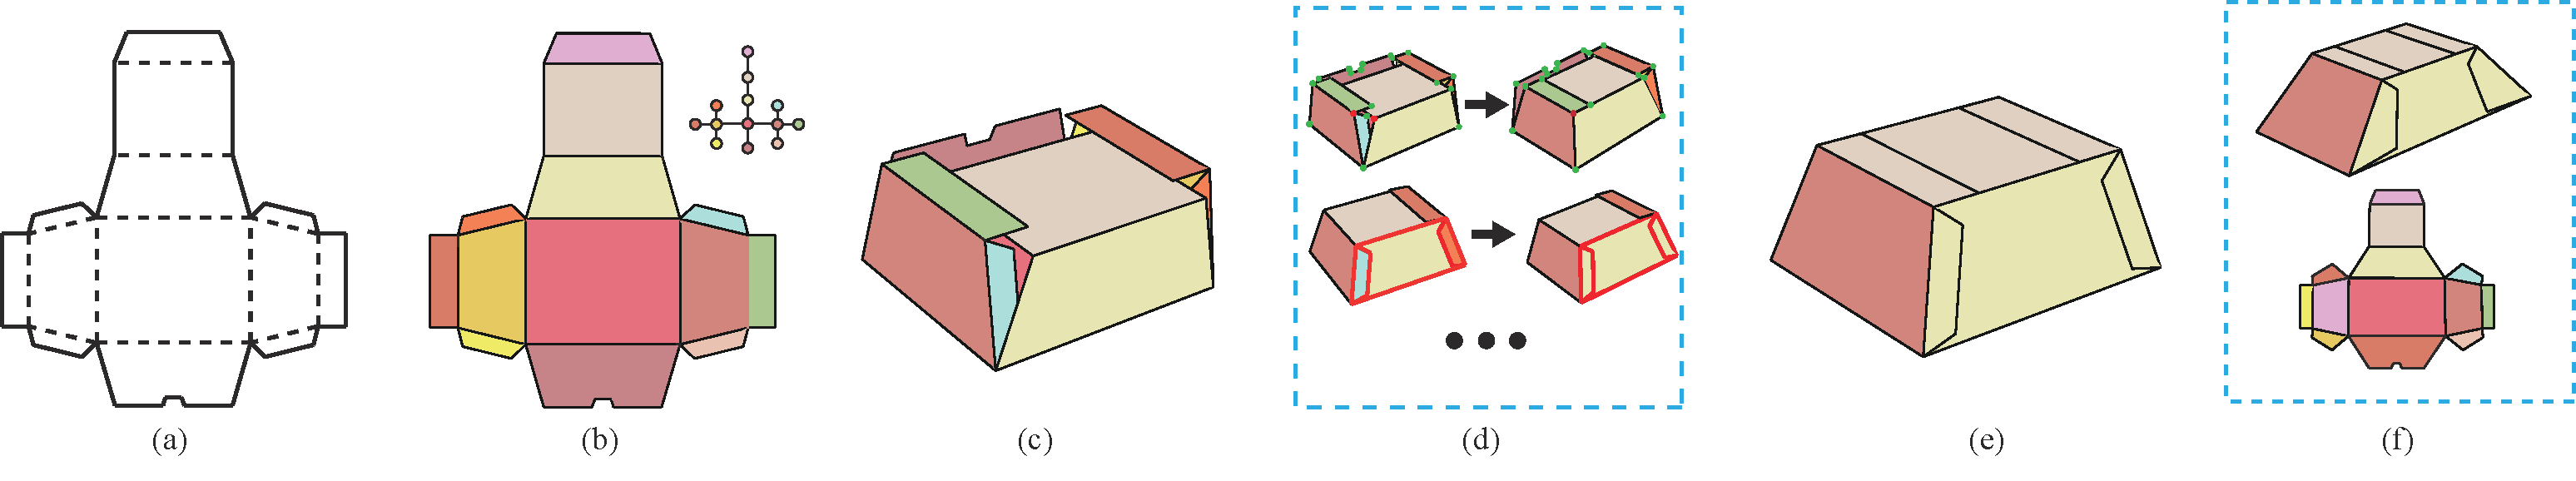
\includegraphics[width=0.9\textwidth]{images/overview}
	\caption{Given a 2D layout (a), we first extract its 2D mesh (b), with different face in different color. By providing each folding edge with a specific angle, we can construct an initial 3D model (c). The final carton model (e) is built through the shape optimization based on the information acquired from user interactions (d).}
	\label{fig:overview}
\end{figure} 

\subsection{Shape optimization}
\reply{The basic idea of our paper is shape optimization by a set of simple algorithms, }
multiple algorithms have been proposed to enforce shape constraints, and have been used successfully for interactive tools and physical simulation~\cite{Botsch:2006:PCP:1281957.1281959,Igarashi:2005:ASM:1186822.1073323}. 
Bouaziz et al.~\cite{Bouaziz:2012:SSD:2346796.2346802} unified a large variety of geometric constraint into one optimization framework, and provided simple, and robust implementation. 
Poranne et al.~\cite{Poranne2013Interactive} described an interactive method to manipulate and optimize polyhedral meshed with constraints with a linear-time algorithm. 
Tang et al.~\cite{Tang:2014:FPM:2601097.2601213} solved constrained equations by Newton-type method in a fast way, and provided an interactive system to model meshed constrained by equalities and inequalities. 
Deng et al.~\cite{Deng2015} developed an interactive tool to explore architectural design with shape constraints, and provided an optimization method to enforce hard constraints and soft constraints at the same time. 

The studies mentioned above focus on the architectural design with constraints, and proposed different solutions, while our constraints do not need satisfy properties like fairness. As a result, we implement the shape optimization by the method introduced in \cite{Bouaziz:2012:SSD:2346796.2346802} for its robustness and simplicity.
%In our paper, we implement the shape optimization by the method introduced in \cite{Bouaziz:2012:SSD:2346796.2346802} for its robustness and simplicity.




\section{Overview}\label{sec:overview}


%Given a 2D expanded layout of a carton, our system allows users to explore the shape and structure of corresponding models.


 
Figure~\ref{fig:overview} shows the overview of our algorithm. 
As shown in Figure~\ref{fig:overview}(a), the input 2D design layout of a carton consists of a set of cutting edges (solid lines) and folding edges (dashed lines).
%
Given the 2D layout, an undirected graph is built and faces are extracted by finding minimum cycles in the graph, as Figure~\ref{fig:overview}(b) shows. 
%Each face is filled with a unique color. %by ignoring the holes in the plane
The 2D layout therefore can be represented by a polymesh $\mathcal{L}=(V,E,F)$, where $V$ is the set of vertexes, $E$ is the set of all edges, and $F$ is the set of faces. 
The edge set $E=E_c\cup E_f$, where $E_c$ is the set of cutting edges, and $E_f$ is the set of folding edges.
%
To build a 3D carton model $\mathcal{M}=(V, E, F)$ from the 2D layout $L$, while they share the same topology, we compute the 3D coordinates of all vertexes in $V$. 
%

However, it is not intuitive to analytically define the desired final 3D shape from a 2D layout. 
One possible way is to detect all the possible geometric constraints such as vertex merging, face parallelism, adjacent face orthogonality, and then to integrate all these possible constraints together to form a large equation system. 
But the challenge is that these local constraints can not well describe complicated and creative designs. 
Moreover, there are many ambiguities when detecting these constraints in a 2D layout that consists of many repeated edges and faces. 
%
We propose a two-step algorithm based on the observation that humans usually fold edges with a right angle to get a rough shape and then merge vertexes or edges to get a stable 3D carton.
% Our algorithm consists of two steps. 
First, an initial 3D model (Figure~\ref{fig:overview}(c)) is constructed based on \cxj{a set of simple rules}{\color{blue}{a specific angle along each fold edge}}, as described in Sec.~\ref{sec:initialization}.
The user can then manipulate and explore 3D shapes of the canton based on a series of suggestive operations provided by our system. 
%
The final model is shown in Figure~\ref{fig:overview}(e).

% is finally built through the optimization based on the information acquired from user interaction. 
\cxj{Modify this overview when you have new figure.}
{\color{blue}{Furthermore, our system allows users modify the final 3D model to the desired shape, and automatically enforce the shape constraints reversely to the flat polymesh to get a deformable layout as shown in Figure~\ref{fig:overview} (f).}}


\comments{
  a flat polymesh $L$ is created from a 2D design layout of a box, then we deform the input polymesh into its 3D realization $R_i$ according to the predicted angles along each of its fold edges, and through optimization, generate final model $R_f$. A polymesh consists of a set of vertices, edges and faces $M = (V,E,F)$, the number of vertexes $V$, edges $E$ and faces $F $ vary from one mesh to another. However, a pair of $(L,R_f)$ as the 2D layout and its corresponding 3D realization share the same topology and therefore they have the same number of vertices, edges and faces. A flat mesh as a 2D layout $L$ has its $z$ component of each vertex set to be a constant zero: $X_z(\mathbf{v}) \equiv 0$ where $X = (X_x,X_y,X_z)$ is the vertex coordinate, and its normal of each face set as $(0,0,1)^T$: $\mathbf{n}(f) \equiv (0,0,1)^T$, where $f \in F$.
}


\begin{figure}
	\centering
	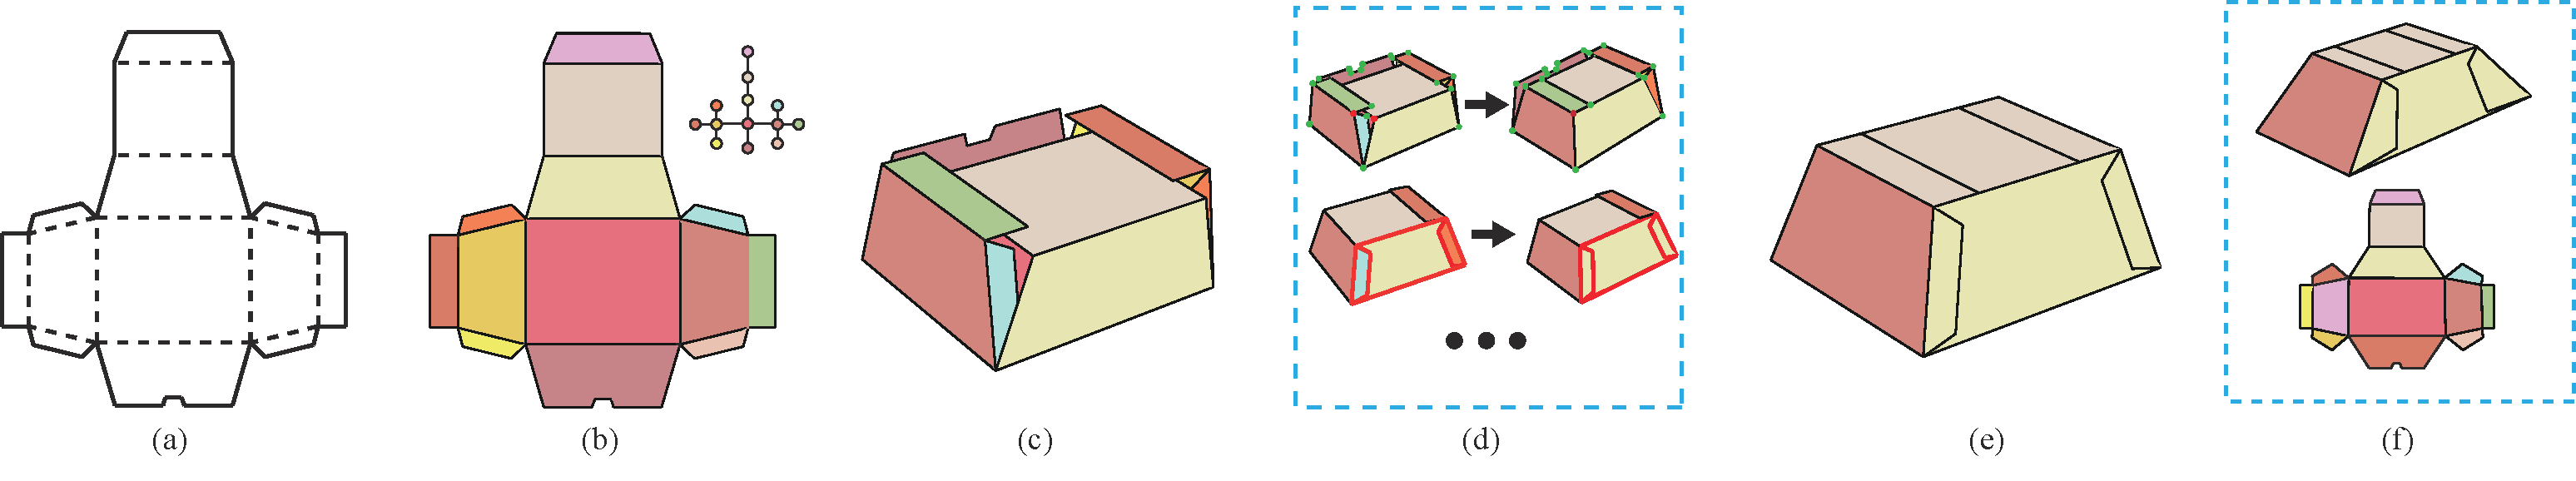
\includegraphics[width=0.9\textwidth]{images/overview}
	\caption{Given a 2D layout (a), we first extract its 2D mesh (b), with different face in different color. By providing each folding edge with a specific angle, we can construct an initial 3D model (c). The final carton model (e) is built through the shape optimization based on the information acquired from user interactions (d). \cxj{update caption for new figure.} {\color{blue}{Our system also allows users to manipulate the 3D model, and explores deformable layout by enforcing geometric constraints reversely to the flat mesh (f). }}}
	\label{fig:overview}
\end{figure} 


\section{Algorithm}\label{sec:optimization}

\comments{
Assuming every face in the carton model is rigid, which means the interior angle in each plane stays the same.  
%
Furthermore, planes are connected by hinges at the boundary of patches, and the planar layout has its front and back.}

In this section, we explain our algorithm in detail. 
Initially, assume that the 2D layout $\mathcal{L}$ lies on the $XOY$ plane, so that each vertex $\mathbf{v}_i(x_i,y_i,z_i)$ in $V$ has $z_i=0$. 
Each face in $F$ has a normal $\mathbf{n}_i=(0,0,1)^T$.
%
In the first step of our algorithm, our system automatically {\color{blue}{folds the original flat mesh into a rough model by assigning a specific angle to each folding edge.}}
%computes the normal of the desired 3D carton based simple rules of orthogonality and parallelism.
In the second step, the carton shape is refined based on a set of potential geometric constraints.



%\cxj{re-write this section. Describe clearly about the parameters, the objective, and methods. }
%In this section we explain the reason why using a specific angle to each fold edge, and constructing our initialized model. 

A general process for humans to fold a carton starts from folding each edge by a rough angle and then connecting close vertexes to obtain a box-like shape. 
Naturally, we first fold the 2D layout by assigning a rotation angle to each pair of adjacent faces to get a rough shape, instead of directly computing the vertex coordinates.
%The basic idea is to interpret the folded state of a box as a series of rotation angles along each edge, and by setting specific value of angles which is $\pi/2$, we can have a rough model to assist the later optimization.
%	
Observed from existing data in the Internet, most of the traditional cartons are cuboid for holding files or delivering daily supplies. 
Although there is a recent trend to design more complicated layouts to attract consumers, the shape of these unusual cartons is similar to boxes as their functions are still packaging commodity. 
%
Therefore, we choose $\pi/2$ as the initial value of the rotation angle to each folding edge. 
%
First, a face graph of a layout is constructed, as shown in Figure~\ref{fig:midresult} (a).
Each face is a node, and there is an edge between two faces if they are connected by a folding edge.
%
The faces in the 2D layout are recursively folded in a breadth-first manner.
Starting from the face with the maximal area, our system folds all its adjacent faces by rotating them around their connecting edge by $\pi/2$, and then continues to others. 
Figure~\ref{fig:midresult} illustrates the folding process of a cuboid carton. 

\begin{figure}[ht]
	\centering
	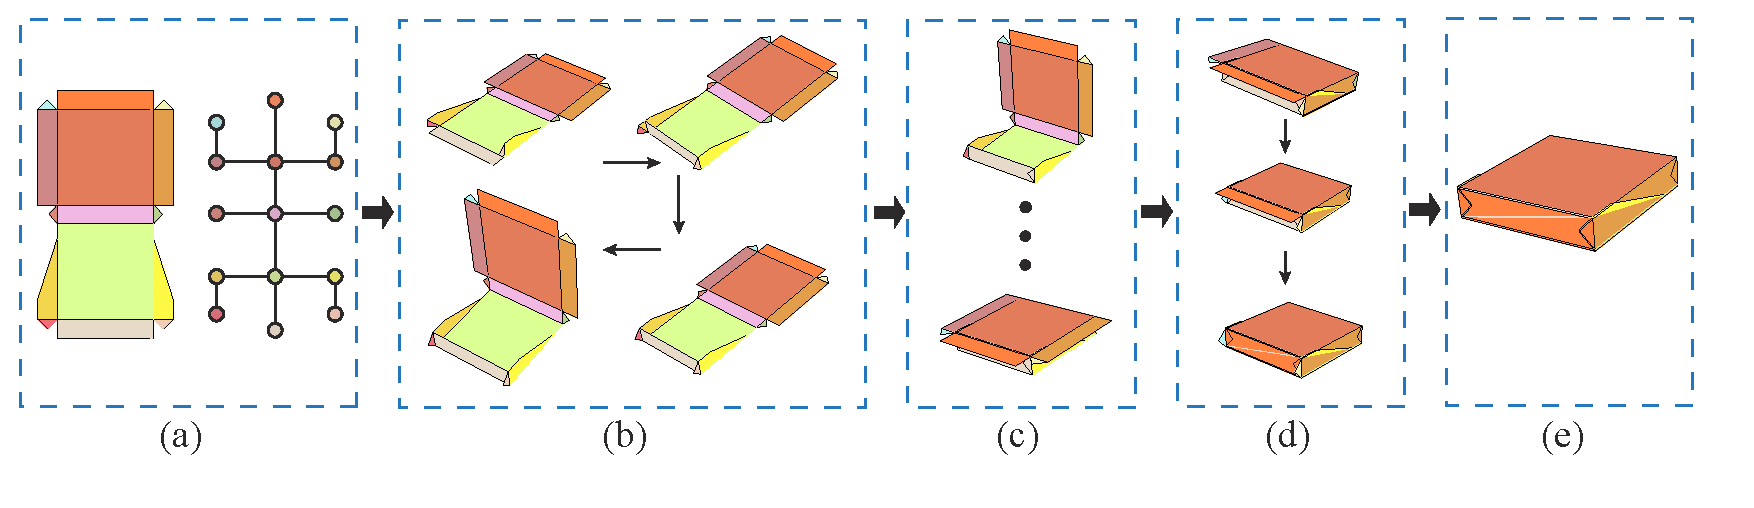
\includegraphics[width=0.9\textwidth]{images/midresult}
	\caption{A rough 3D shape is obtained by folding each face by $\pi/2$ in the 2D layout (a) in a breadth-first manner, starting from the face with the maximal area. (b), (c), (d) and (e) are the different folding stages in the initialization step.}
	\label{fig:midresult}
\end{figure}


{\color{blue}{The following two figures}} shows a group of results generated by simply folding faces by $\pi/2$.
Traditional cartons in cuboid shapes could reach an ideal state, as Figure~\ref{fig:initial-automatic} shows.
However, many complicated designs still need refinement, such as the four examples in Figure~\ref{fig:initial-need-improvement}. 
Take the hexagonal box as an example, the 3D model can be improved by simply snapping the small paste faces to its nearby faces. %
%
As a result, we provide an suggestive interface by automatically detecting potential geometric modifications in the rough carton shape for users to explore.
%interactively allow users to add these constrains into our system and optimize to a desired model, as described in the following section.

\begin{figure}
	\centering
	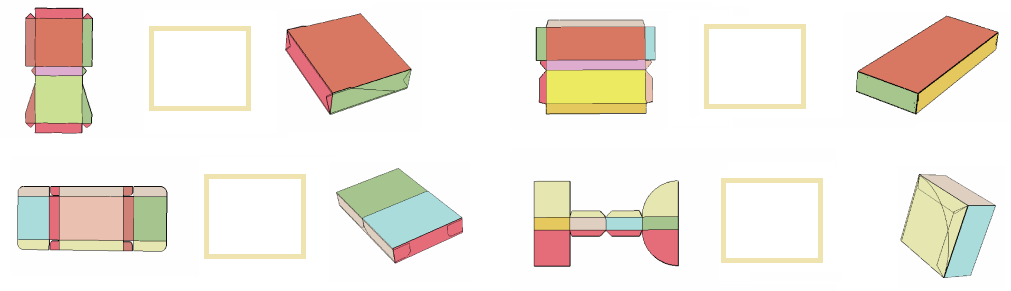
\includegraphics[width=0.9\textwidth]{images/initial-auto.png}
	\caption{Four examples of carton models that can be fully automatically generated from 2D layouts by folding each edge with a fixed angle $\pi/2$. }
	\label{fig:initial-automatic}
\end{figure}


\begin{figure}
	\centering
	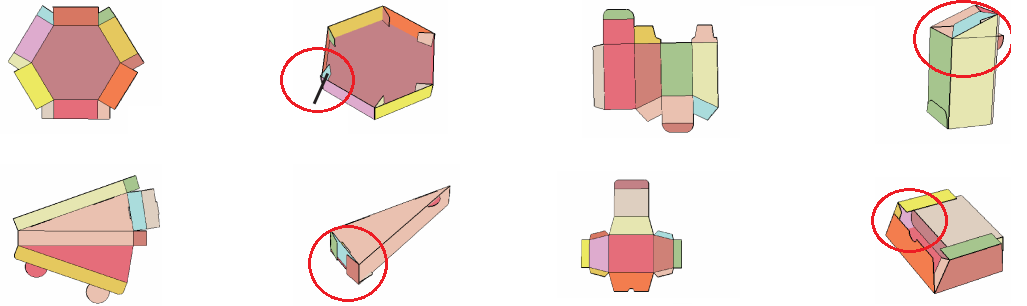
\includegraphics[width=0.9\textwidth]{images/initial-improve.png}
	\caption{Four examples of the carton models that need shape improvement. While the shapes are not cuboid, using a fixed angle $\pi/2$ leads to non-closed shape and loose structure. }
	\label{fig:initial-need-improvement}
\end{figure}
%%%%%%%%%%%%%%%%%%%%%%%%%%%%%%%%%%%%%%%%%%%%%%%%%%%%%%%%%%%%%%%%%%%%%


\cxj{It is not clear how do you assign the angle $\pi/2$ to all angles. What order do you use? Show the mid-stage? any problem need to discuss? }

\subsection{Shape Refinement}\label{sec:refinement}

%there is still a need to refine the results that have not folded into pleasing results. 
Though not perfect, the initial 3D shape provides a good start point for generating the final carton model. 
%
To further refine the 3D shape, the 3D coordinates of all the vertexes are then computed based on a set of shape constraints.
%
%the main idea is to prescribe the shape constrains by a set of vertexes of the polymesh. 
Moreover, with the extra information acquired from user interaction, we can finally construct the desired 3D realization.
In this step, the coordinate of vertexes are chosen as our objective instead of angles on folding edges.
This is mainly because that the geometric constrains in the 3D shape can be more simply and intuitively represented by 3D vertexes.
% and we can implement the algorithm introduced by Bouaziz et al. easily~\cite{Bouaziz:2012:SSD:2346796.2346802}.
 

%\subsection{Aided Detection}

%While the initial 3D model with simple angle folding provides a rough idea about the carton shape, 
Our system  automatically detects a group of possible shape constraints to form the final 3D model, such as vertex merging, shape symmetry, and so on. 
%
These guiding operations are provided to the user at bottom of the user interface, for the user to quickly select and explore the carton shapes.
In our system, \cxj{two} types of shape refinement operations, vertex merging, and shape symmetry, are automatically detected.

%
%In order to assist users construct the final carton interactively, we also provide symmetry detection and merging points detection to improve the efficiency of constructing models .

\noindent
\textbf{Vertex merging} is detected among the nearby vertexes. 
For irregular shapes consists of non-rectangular faces or non-perpendicular adjacent faces, some vertexes supposed to folded to the same position are close to each other after the initialization step. 
For each pair of vertexes $\mathbf{v}_a$, $\mathbf{v}_b$ {\color{blue}{that in the nonadjacent face}}, if $|\mathbf{v}_a-\mathbf{v}_b|<\epsilon$, and one edge connecting to $\mathbf{v}_a$ has the same length with one edge connecting to $\mathbf{v}_b$.
\cxj{Add discussion about more than two vertexes. Improve figure by highlighting the merging edge and vertex. }
{\color{blue}{While there are sometimes more than two vertexes that need to be merged, as an example shown in Figure~\ref{fig:suggestion} (a), after $\mathbf{v}_a$ and $\mathbf{v}_b$ being considered to relocate in the same place, if the next vertex $\mathbf{v}_c$} is detected satisfying $|\mathbf{v}_c-\mathbf{v}_a(\mathbf{v}_b)|<\epsilon$ and one of incident edges of $\mathbf{v}_c$ has the same length as $\mathbf{v}_a(\mathbf{v}_b)$'s, vertex $\mathbf{v}_c$ also has the need to merge with $\mathbf{v}_a$ and $\mathbf{v}_b$.}

%Consider the initialization results can represent the ideal model partly, the disadjacent vertices that have one edge with same length can be regarded as targets that need to be located in the same place if their Euclidean distance is below a certain threshold.

\noindent
\textbf{symmetry detection} {\color{blue}{focus on the symmetry property of vertexes. $\mathbf{v}_a$ and $\mathbf{v}_b$ are regarded as symmetric pair, if for each pair of $l_{ai} \in \{ l_{a1},l_{a2}...l_{am}\}$ and $l_{bi} \in \{ l_{b1},l_{b2}...l_{bn}\}$, $m = n$ and $|l_{ai}- l_{bi}|<\epsilon$ where $m$ is the number of $\mathbf{v}_a$'s ordered set of the incident edges' length $\{ l_{a1},l_{a2}...l_{am}\}$, and $n$ is the number of $\mathbf{v}_b$'s ordered set of the incident edges' length $\{ l_{b1},l_{b2}...l_{bn}\}$.
		
 When involving multiple vertexes, the searching criterion is based on symmetric vertex pair detection described above. The symmetric vertex set of selected vertexes $\{\mathbf{v}_1,\mathbf{v}_2,...,\mathbf{v}_{n-1}\}$ is $\{\hat{\mathbf{v}}_1,\hat{\mathbf{v}}_2,...,\hat{\mathbf{v}}_{n-1} \}$, the vertex set $\{\mathbf{v}_1,\mathbf{v}_2,...,\mathbf{v}_n\}$ has the symmetric vertex set $\{\hat{\mathbf{v}}_1,\hat{\mathbf{v}}_2,...,\hat{\mathbf{v}}_n \}$, if $||\mathbf{v}_n-\mathbf{v}_i| - |\hat{\mathbf{v}}_n-\hat{\mathbf{v}_i}||<\epsilon$, for $i = 1,....,n-1$.}} 

%On account of the simplicity of the carton shape, the vertexes that have same length set of incident edges can be regarded as symmetric pair. While users select vertexes that need to be merged together, symmetry detection can reduce repetitive work by giving users suggestions of symmetric vertexes.
\cxj{Describe your algorithm first. Then explain fig 5 as a specific example.}

\cxj{Add a figure to illustrate this. }
{\color{blue}{Take Figure~\ref{fig:suggestion} (b) as an example, after users selecting vertexes circled in red, our system can automatically detect their symmetric set circled in blue. As an result, our system can detect these symmetry pairs to assist users improve efficiency.}}

\begin{figure}
	\centering
	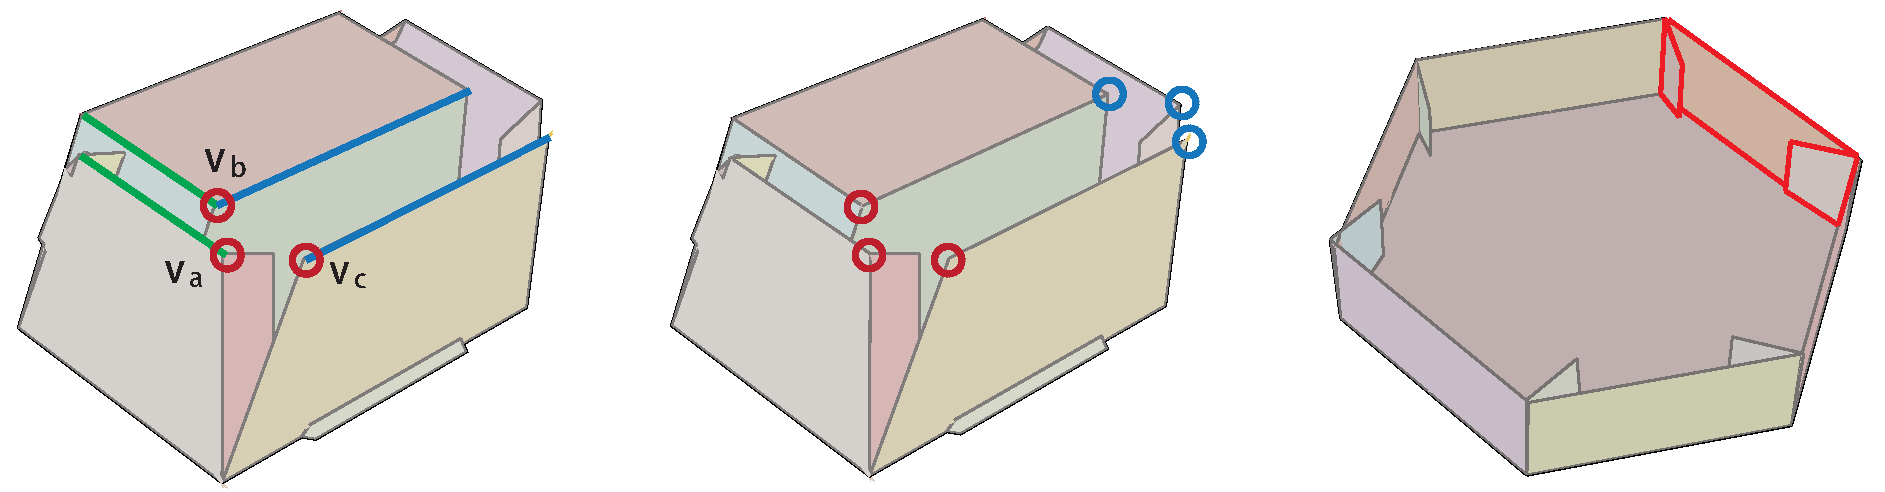
\includegraphics[width=0.9\textwidth]{images/suggestion}
	\caption{Vertex merging detection is well illustrated by (a), $\mathbf{v}_a$ and $\mathbf{v}_b$ may have the need to merge cause $|\mathbf{v}_a-\mathbf{v}_b|<\epsilon$, and one edge connecting to $\mathbf{v}_a$ marked as green has the same length with one edge connecting to $\mathbf{v}_b$ also marked as green. $\mathbf{v}_c$ can also be considered that need to merge with $\mathbf{v}_a$ and $\mathbf{v}_b$ as $|\mathbf{v}_c-\mathbf{v}_a(\mathbf{v}_b)|<\epsilon$ and one of incident edges of $\mathbf{v}_c$ marked as blue has the same length as $\mathbf{v}_a(\mathbf{v}_b)$'s also marked as blue. While users select three vertexes circled in red (b), our system can detect symmetric vertexes circled in blue automatically. \cxj{show more possible suggestions in this figure. Make sure the font in consistent with the caption}.\cxj{the font of a, b is too big. Is this automatically detected result?}}
	\label{fig:suggestion}
\end{figure}

\cxj{Once the user selects a suggested shape refinement operation, we optimize the 3D shape based on a series of geometric constraints.}
%We now introduce the constrains used in our construction method:
Given the current mesh whose vertex positions are defined as $\{\vo_i\}^{N}_{i=1}$, a new mesh with the same topology but new vertex positions $\{\vn_i\}^{N}_{i=1}$ is constructed.
%
The geometric constraints can be classified into two groups, basic geometric constraints and user-selected constraints. 
First, to keep the geometric shape of each face, the constraints including edge length constraint, coplanarity, and face rigidity, which are corresponding to similarity constraint and plane constraint described in \cite{Bouaziz:2012:SSD:2346796.2346802}. 

\noindent
\textbf{Edge length constraint} 
For each edge $\{e_j\}_{j=1...M}$, its length should be preserved when refine the carton shape.
Hence, its two endpoints $\mathbf{v}_{js}$ and end point $\mathbf{v}_{jt}$ should satisfy 
\begin{equation}
||\mathbf{v}_{js} - \mathbf{v}_{jt}||^2 = ||\mathbf{\hat{v}}_{js} - \mathbf{\hat{v}}_{jt}||^2.
\label{equ:edge}
\end{equation}
%to ensure that the length of each edge stays the same.

\noindent
\textbf{Coplanarity} {\color{blue}{For each face $\{p_k\}_{k=1 \dots P}$, this constraint specifies the face's vertexes should always lie on a plane. We can compute the sorted eigenvectors $\mathbf{U} = [\mathbf{e}_1, \mathbf{e}_2, \mathbf{e}_3]$ of the $ 3 \times 3$ covariance matrix $\mathbf{C}^T\mathbf{C}$ where $\mathbf{C} = \{\mathbf{v}_{kj}\}_{j=1}^{N_k}$, $\mathbf{v}_{kj}$ is the $j$th vertex among $N_k$ vertexes in face $p_k$}. Plane projection can be obtained by removing the last column of $\mathbf{U}$. }
%For each face $\{p_k\}_{k=1 \dots P}$ and its normal $\mathbf{n}_k$, each line connected by two points $\mathbf{v}_{ka}, \mathbf{v}_{kb}$ on the plane is perpendicular to the normal. 
\cxj{where do you get the face nornal in the refined shape?}

\noindent
\textbf{Face rigidity} For each face $\{p_k\}_{k=1 \dots P}$, the length of each line connecting two non-adjacent points $\mathbf{v}_{ka}, \mathbf{v}_{kb}$ on the plane remains the same, so that the shape of each plane keeps unchanged.
\begin{equation}
||\mathbf{v}_{ka} - \mathbf{v}_{kb}||^2 = ||\hat{\mathbf{v}}_{ka} - \hat{\mathbf{v}}_{kb}||^2.
\label{equ:plane}
\end{equation}

The information acquired from user interaction will add enough constrains to solve the optimization problem, and one of the interaction is to choose the right given suggestion including points needed to be merged together. As for the point information, the constrains can be written like:

\noindent
\textbf{Merging vertexes} For any two vertexes $\mathbf{v}_p$ and $\mathbf{v}_q$ that are selected to be merged as the same vertex, we have 
\begin{equation}
\mathbf{v}_p - \mathbf{v}_q = 0.
\label{equ:point}
\end{equation}
%if these two points $\mathbf{v}_p$, $\mathbf{v}_q$ need to be moved into the same place.
\cxj{shape symmetry?}


When the above constrains still lead to an ill-posed problem, soft constraints will be added to keep the original positions of irrelevant vertexes. 


\noindent
\textbf{Irrelevant vertexes} $\{\mathbf{v}_i\}$ which are not in the same plane with $\mathbf{v}_p$ or $\mathbf{v}_q$, should be stay at their original location. 
We add these soft constraints by adding a small weight $w$, which is set 0.001 in our experiments. 
\begin{equation}
\mathbf{v}_i - \mathbf{\hat{v}}_i = 0.
\label{equ:irrelevant}
\end{equation}

Figure~\ref{fig:constrain} illustrates the necessity of basic three constrains.
\cxj{More detailed explaination on the figure. Explain the three constraints in the figure.}
{\color{blue}{When we merge three vertexes circled in red Figure~\ref{fig:constrain} (b) into one location, the optimized model is generated under basic constraints shown in Figure~\ref{fig:constrain}}. The model shown in Figure~\ref{fig:constrain} (d) (e) and (f) are the results after optimizing without edge length constrain, coplanarity and face rigidity constrain separately. Without edge length constrain, the two red edges have been stretched Figure~\ref{fig:constrain} (d), the face surrounded by red lines Figure~\ref{fig:constrain} (e) is not a standard plane without coplanarity, and the face surrounded by red lines in Figure~\ref{fig:constrain} (f) has been deformed without face rigidity.}

\begin{figure}
	\centering
	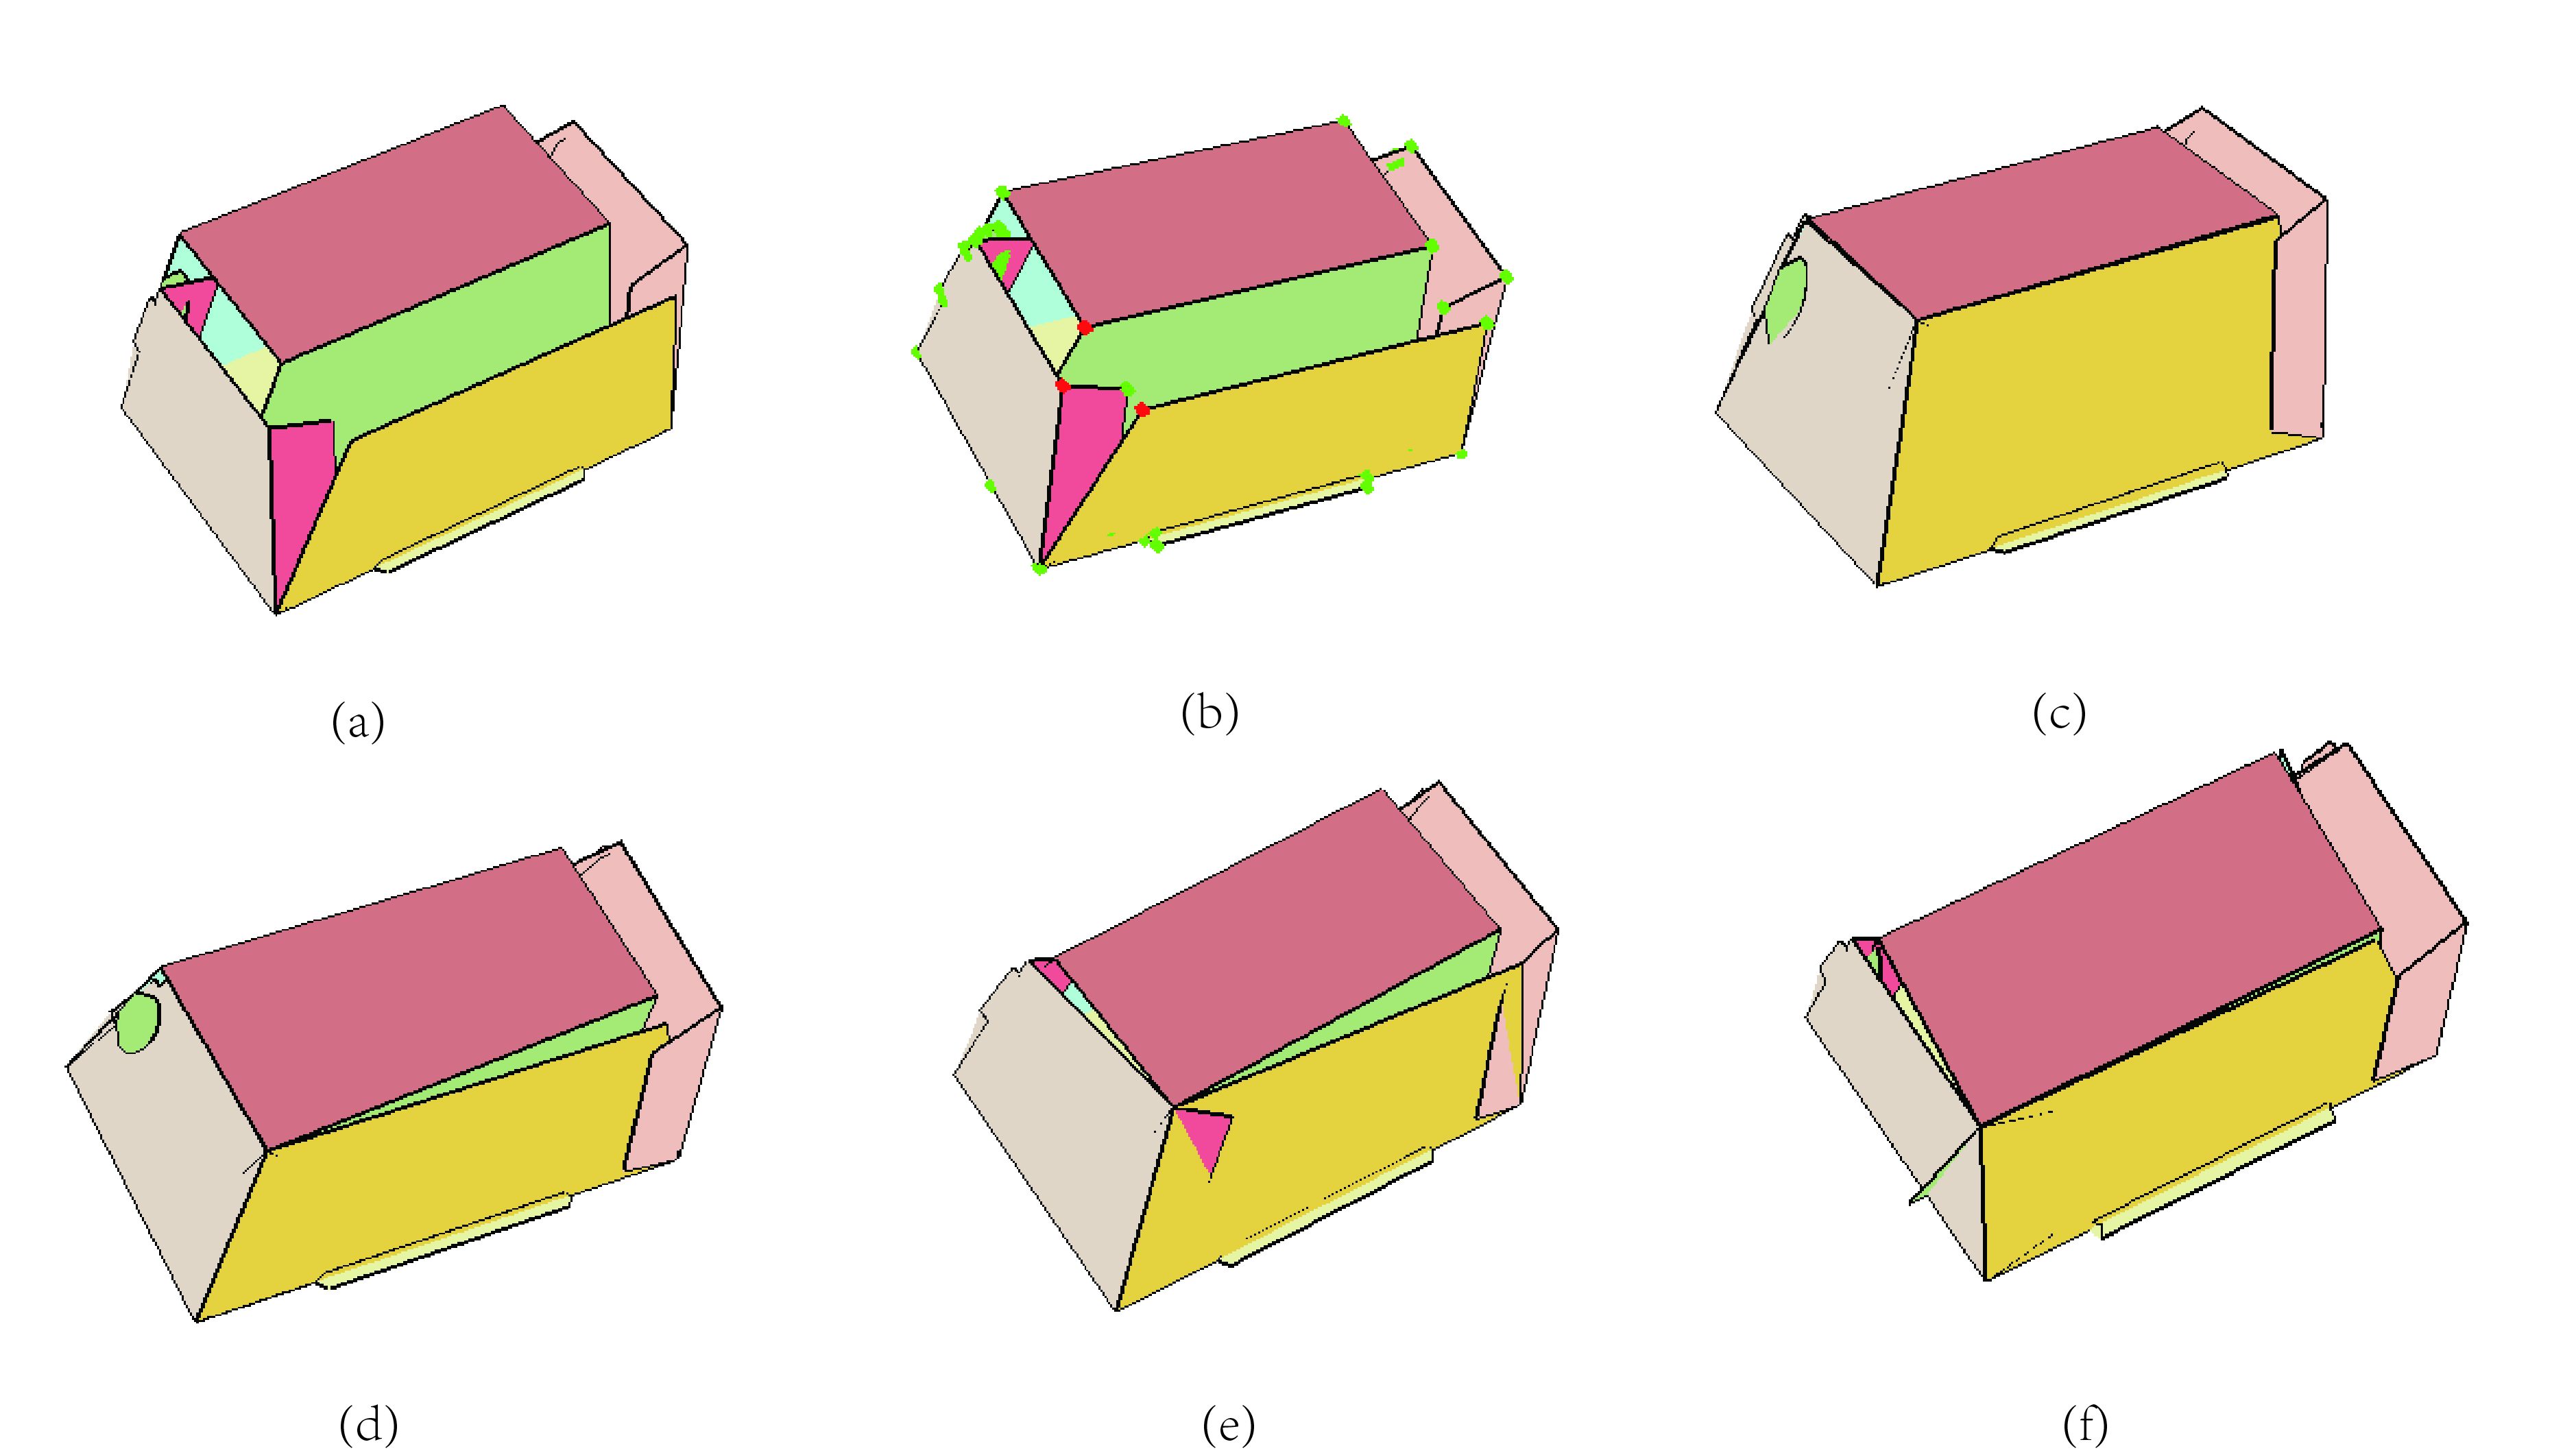
\includegraphics[width=0.9\textwidth]{images/constrain.jpg}
	\caption{Given an initial state~(a), by choosing three points marked in red~(b) that need to be relocated together, basic three shape constrains can lead to the optimization result~(c). The bottom three are the results optimized lack of edge length constrain, coplanarity and face rigidity separately, compared to~(c), the results can not keep the basic shape well. Without edge length constrain, the two red edges have been stretched (d), the face surrounded by red lines (e) is not a standard plane without coplanarity, and the face surrounded by red lines in (f) has been deformed without face rigidity.}
	\label{fig:constrain}
\end{figure}


\section{Suggestive Interface for Shape Modification }\label{sec:interaction}
%
For some creative designs, the rough 3D carton model generated based on our heuristic approach still needs some improvement or the user might edit the carton shape. 
%After folding the flat layout into a rough shape, we need to refine the model to final state through basic geometric constraints and user-selected constraints which are obtained from user interaction. 
To assist users to refine the carton model, our system is equipped with a set of smart shape refinement operations, such as automatically detecting vertexes that can be merged, propagating modification to similar groups, and providing suggestions for users to explore. 
%
While a user edits the carton model in 3D space, which is more intuitive, our system is capable of revising the 2D layout automatically. 

%Figure~\ref{fig:interface} illustrates two operations that the system provides, the first one is selecting points need to be merged by users and the second is select the right option from results by vertex merging detection.   

%\begin{figure}
%	\centering
%	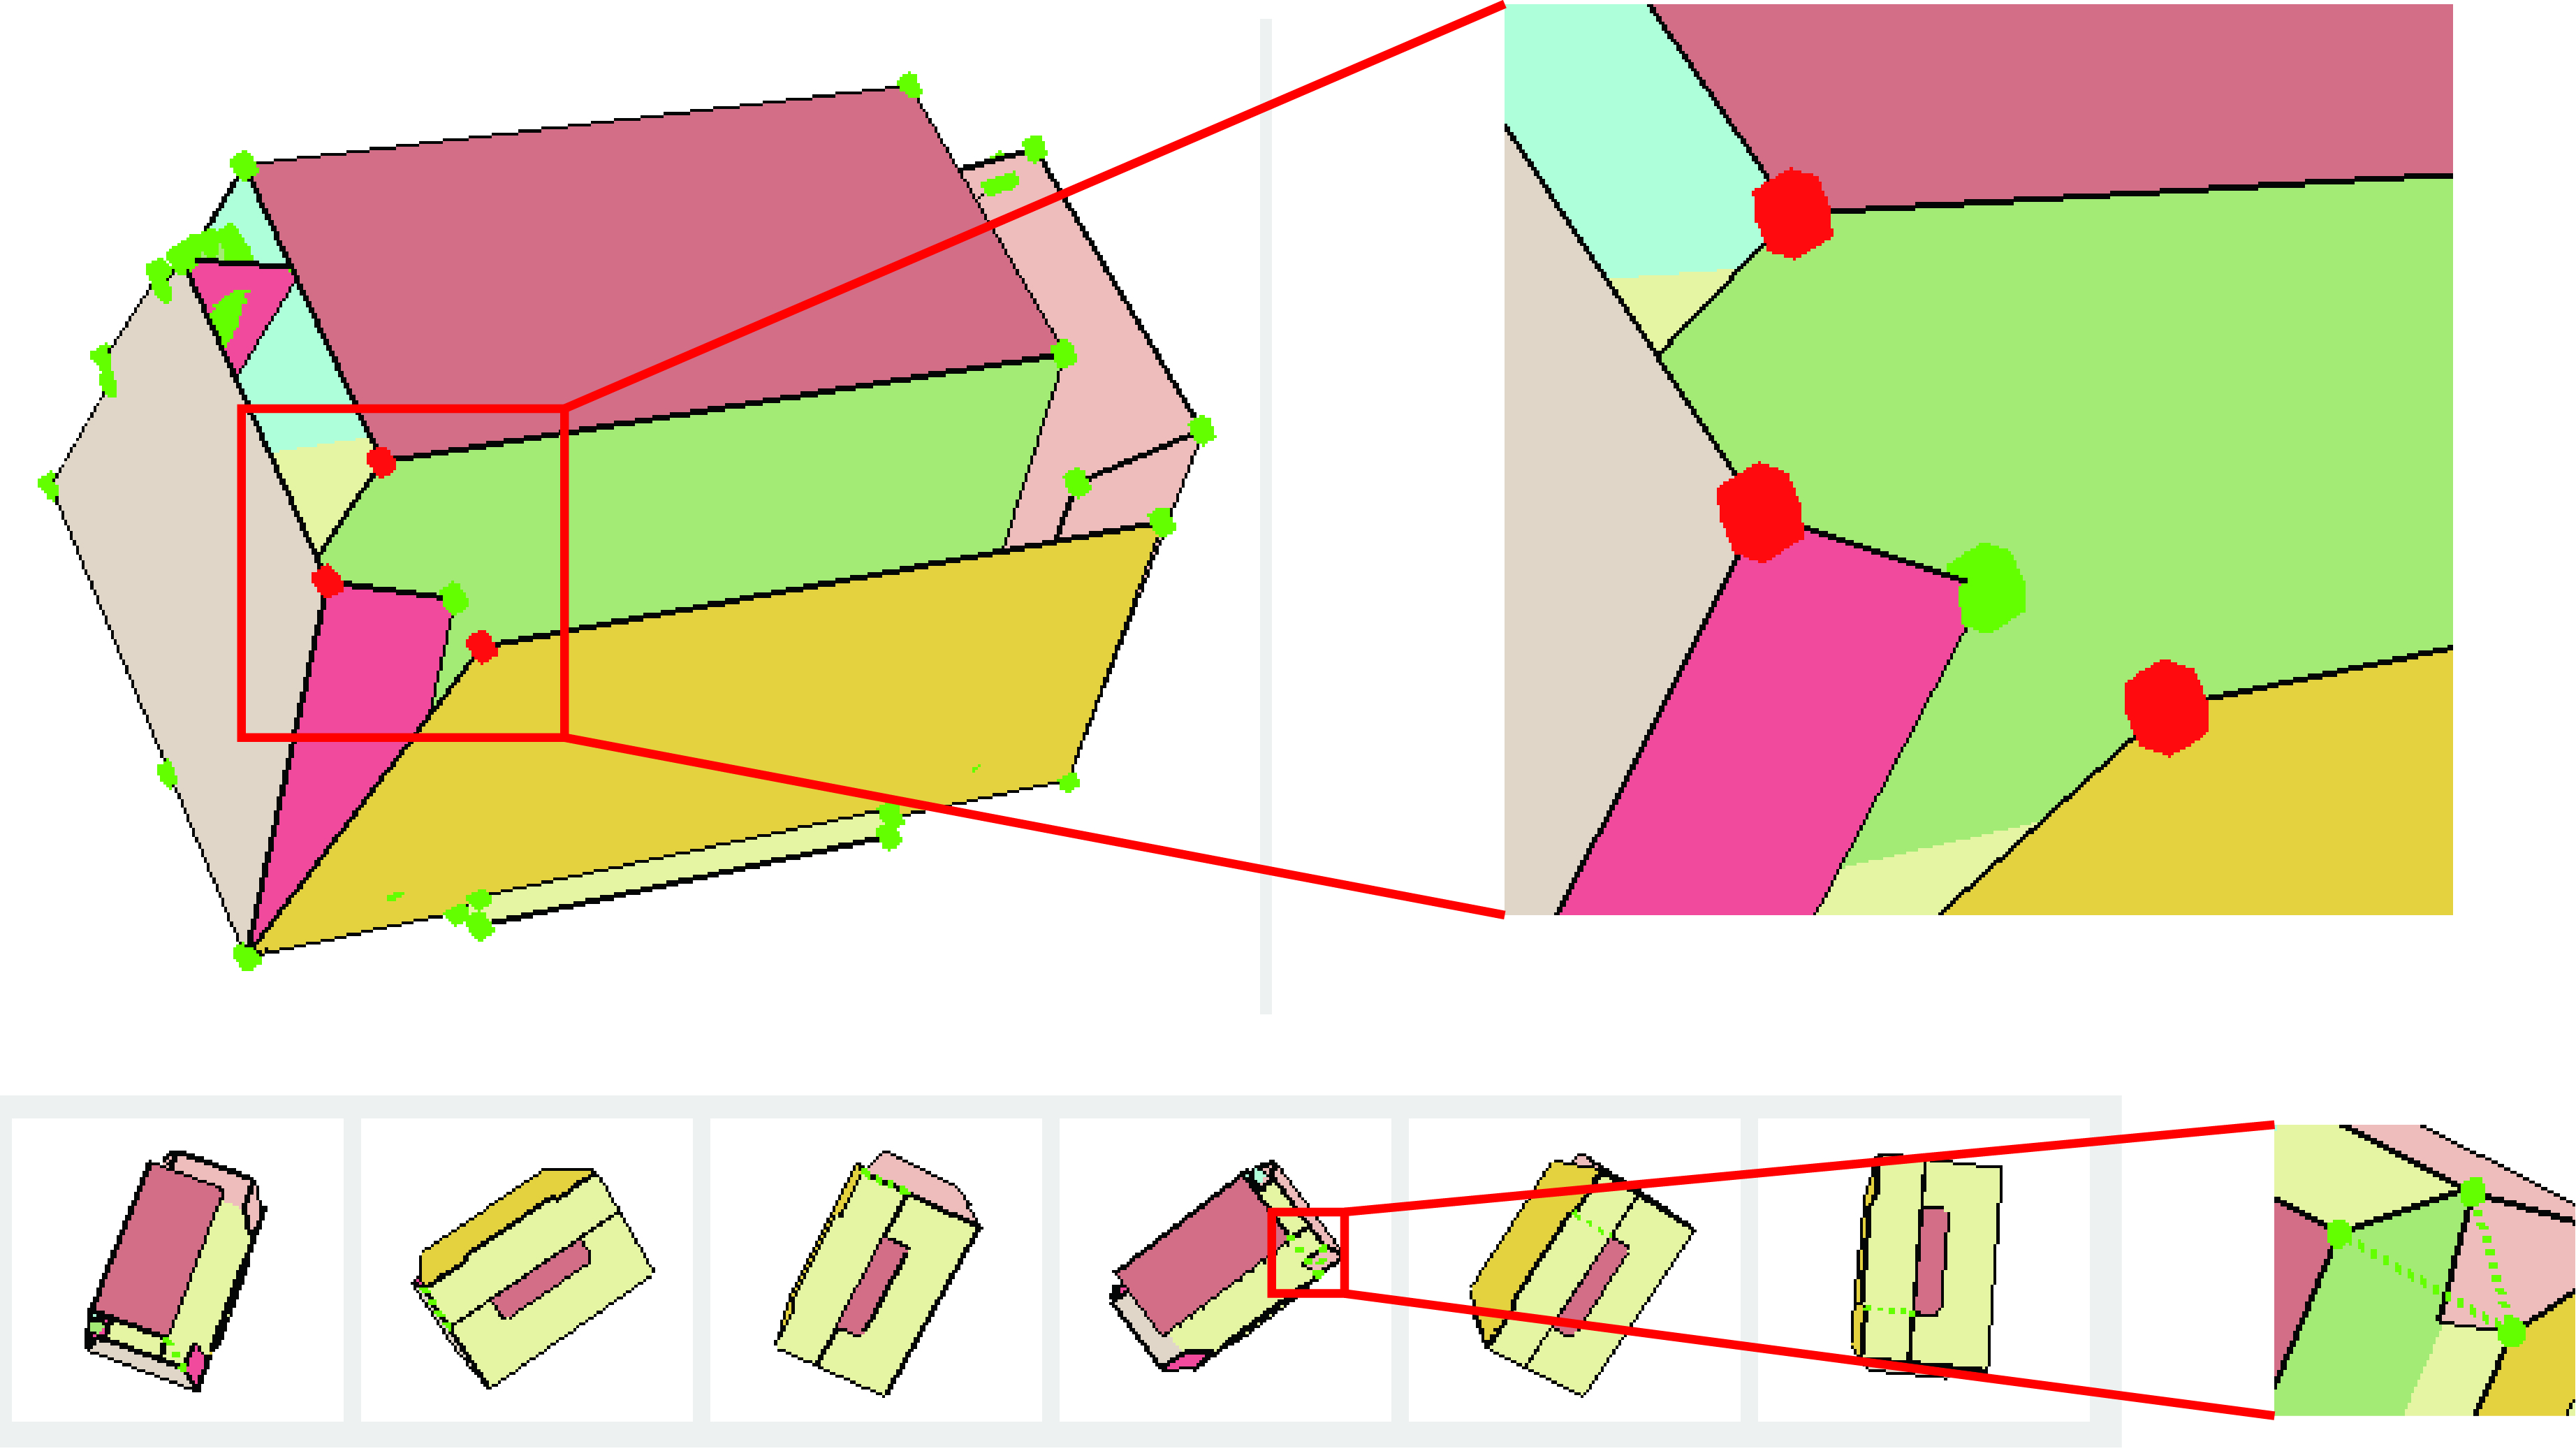
\includegraphics[width=0.9\textwidth]{images/UIdetail.jpg}
%	\caption{two operations that the system provides}
%	\label{fig:interface}
%\end{figure}

\subsection{Suggestive Interaction}

Our system automatically detects a group of potential shape constraints to improve the 3D carton model.
%
These guiding constraints are provided to the user for quickly selecting and manipulating the carton shape.
In our system, three types of shape refinement operations, vertex merging, merging propagation, and face pasting, are automatically detected.

%
%In order to assist users construct the final carton interactively, we also provide symmetry detection and merging points detection to improve the efficiency of constructing models .

\paragraph{Vertex Merging.} 
For irregular shapes which consist of non-rectangular faces or non-perpendicular adjacent faces, some vertexes are close to each other after the initialization step.
A practical carton model can be obtained by simply merging these nearby vertexes together if their have coherent edges.
%
Any pair of vertexes $\mathbf{v}_a$, $\mathbf{v}_b$ in different faces is detected as mergeable, if $|\mathbf{v}_a-\mathbf{v}_b|<\epsilon$, and there is an edge connecting to $\mathbf{v}_a$ having the equal length with one edge connecting to $\mathbf{v}_b$,
%
$\epsilon$ is a distance threshold and set as 50mm in our experiments.
More vertexes can be merged together, as shown in Figure~\ref{fig:suggestion:a} by gradually adding one vertex $\mathbf{v}$ each time if $\mathbf{v}$ is mergeable with at least one vertex in current list. 
%Consider the initialization results can represent the ideal model partly, the disadjacent vertices that have one edge with same length can be regarded as targets that need to be located in the same place if their Euclidean distance is below a certain threshold.

\paragraph{Merging Propagation.} %{\color{blue}{focus on the symmetry property of vertexes.
Once the user makes a decision to merge a subset of vertexes $\mathbb{V}=\{\mathbf{v}_i\}_{i=1,\ldots,K}$ from automatic system suggestions, or manually selection, our system will detect if there exists another subset of vertexes $\vset_b$ symmetric to $\mathbb{V}$ and propagate the merging operation to $\vset_b$, as shown in Figure~\ref{fig:suggestion:b}. 
A subset $\mathbb{V}_b$ is symmetric to $\mathbb{V}_a$ if $|\vset_a|=|\vset_b|$, and there exists one-to-one correspondence between the vertexes in $\vset_a$ and $\vset_b$. 
Here, $|\vset|$ is the number of vertexes in a vertex subset $\vset$. 
Two vertexes $\vn_a$ and $\vn_b$ are defined as corresponding vertexes if they have the same number of edges and one-to-one correspondence can be found between the edge lengths. 

\begin{figure}
	\centering
	 \subfigure[Vertex Merging]{
	 	\label{fig:suggestion:a} %% label for first subfigure
	 	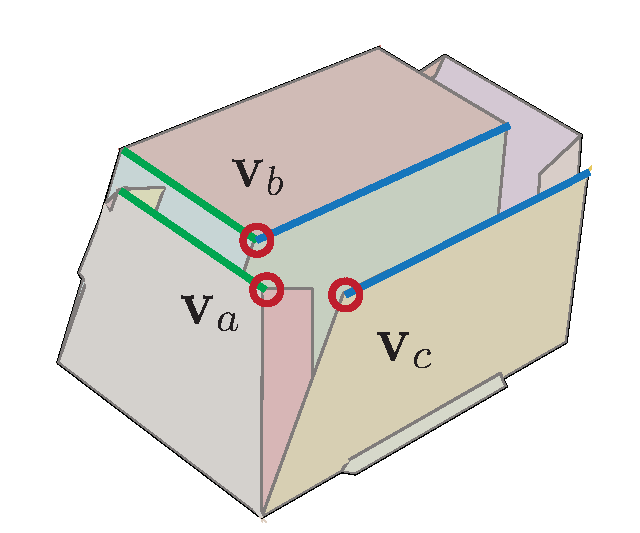
\includegraphics[width=0.3\textwidth]{images/suggestiona.pdf}}
	 \hfill
	 \subfigure[Merging Propagation]{
	 	\label{fig:suggestion:b} %% label for second subfigure
	 	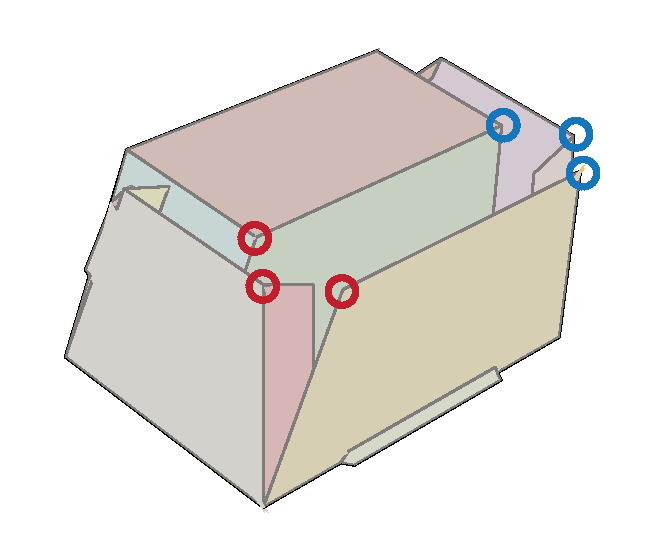
\includegraphics[width=0.3\textwidth]{images/suggestionb.pdf}}
	 \hfill
	 \subfigure[{Face Pasting}]{
	 	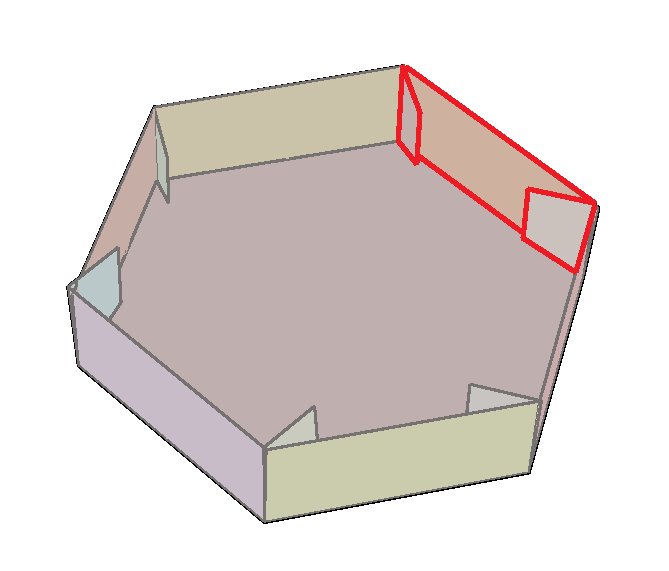
\includegraphics[width=0.3\textwidth]{images/suggestionc.pdf}
	 	\label{fig:facepasting}
	 	}
	 
	 \caption{Three different suggestions on shape modification. (a) A group of vertexes (marked in red) are detected as mergeable. $\mathbf{v}_a$ and $\mathbf{v}_b$ are close to each other and one edge connecting to $\mathbf{v}_a$ has the same length with one edge connecting to $\mathbf{v}_b$ (green edges). $\mathbf{v}_c$ is also considered to be merged with $\mathbf{v}_a$ and $\mathbf{v}_b$ because $\mathbf{v}_c$ is close to $\mathbf{v}_b$ and one edge of $\mathbf{v}_c$ has the same length as $\mathbf{v}_b$ (blue edges). (b) Once the user confirms a suggested vertex merging operation, our system automatically proposes a symmetric group of vertexes that can be also merged (marked in blue). (c) If faces marked in red are detected close to each other and the same with their normals, our system suggests these faces can be sticked together.}
	 \label{fig:suggestion}
\end{figure}

%\begin{figure}
%	\centering
%	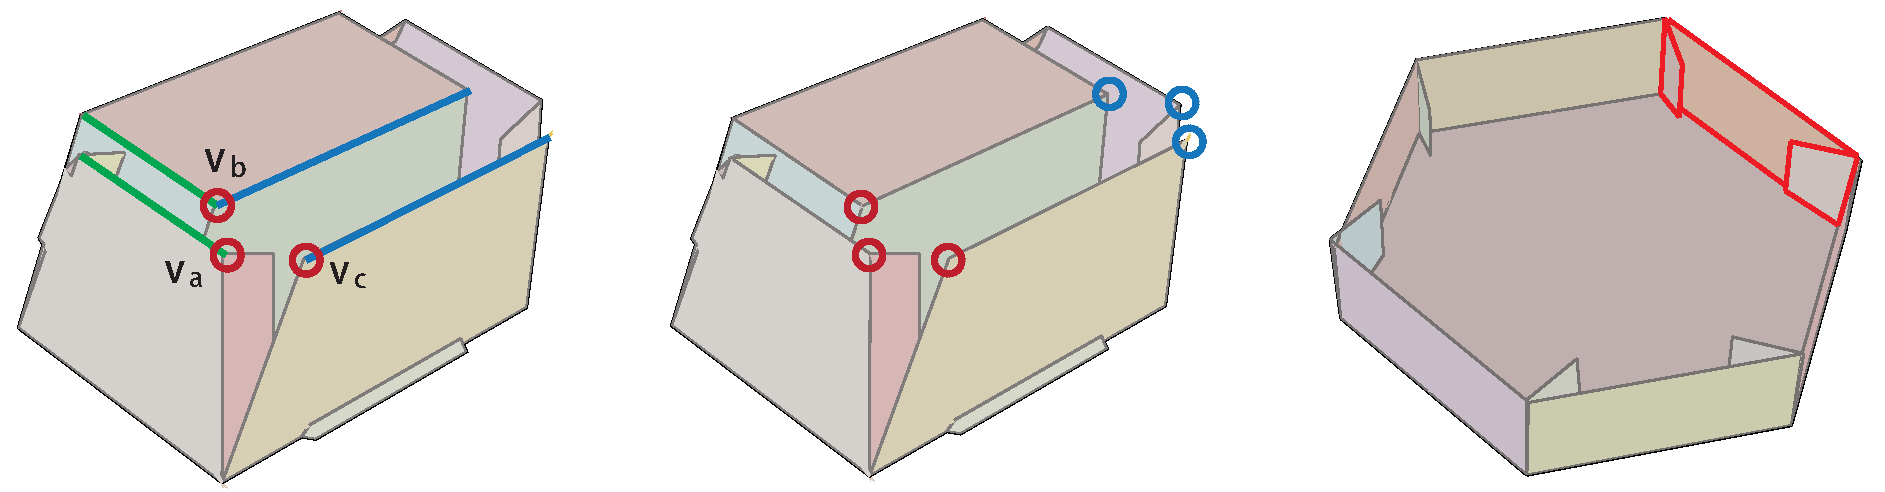
\includegraphics[width=0.9\textwidth]{images/suggestion}
%	\caption{Vertex merging detection is well illustrated by (a), $\mathbf{v}_a$ and $\mathbf{v}_b$ may have the need to merge cause $|\mathbf{v}_a-\mathbf{v}_b|<\epsilon$, and one edge connecting to $\mathbf{v}_a$ marked as green has the same length with one edge connecting to $\mathbf{v}_b$ also marked as green. $\mathbf{v}_c$ can also be considered that need to merge with $\mathbf{v}_a$ and $\mathbf{v}_b$ as $|\mathbf{v}_c-\mathbf{v}_a(\mathbf{v}_b)|<\epsilon$ and one of incident edges of $\mathbf{v}_c$ marked as blue has the same length as $\mathbf{v}_a(\mathbf{v}_b)$'s also marked as blue. While users select three vertexes circled in red (b), our system can detect symmetric vertexes circled in blue automatically. \cxj{show more possible suggestions in this figure. Make sure the font in consistent with the caption}.\cxj{use subfigure?}}
%	\label{fig:suggestion}
%\end{figure}

\comments{
	$\mathbf{v}_a$ and $\mathbf{v}_b$ are regarded as symmetric pair, if for each pair of $l_{ai} \in \{ l_{a1},l_{a2}...l_{am}\}$ and $l_{bi} \in \{ l_{b1},l_{b2}...l_{bn}\}$, $m = n$ and $|l_{ai}- l_{bi}|<\epsilon$ where $m$ is the number of $\mathbf{v}_a$'s ordered set of the incident edges' length $\{ l_{a1},l_{a2}...l_{am}\}$, and $n$ is the number of $\mathbf{v}_b$'s ordered set of the incident edges' length $\{ l_{b1},l_{b2}...l_{bn}\}$.
	
	When involving multiple vertexes, the searching criterion is based on symmetric vertex pair detection described above. The symmetric vertex set of selected vertexes $\{\mathbf{v}_1,\mathbf{v}_2,...,\mathbf{v}_{n-1}\}$ is $\{\hat{\mathbf{v}}_1,\hat{\mathbf{v}}_2,...,\hat{\mathbf{v}}_{n-1} \}$, the vertex set $\{\mathbf{v}_1,\mathbf{v}_2,...,\mathbf{v}_n\}$ has the symmetric vertex set $\{\hat{\mathbf{v}}_1,\hat{\mathbf{v}}_2,...,\hat{\mathbf{v}}_n \}$, if $||\mathbf{v}_n-\mathbf{v}_i| - |\hat{\mathbf{v}}_n-\hat{\mathbf{v}_i}||<\epsilon$, for $i = 1,....,n-1$.
}

\comments{Take Figure~\ref{fig:suggestion} (b) as an example, after users selecting vertexes circled in red, our system can automatically detect their symmetric set circled in blue. As an result, our system can detect these symmetry pairs to assist users improve efficiency.}

\paragraph{Face Pasting.} Merging vertexes sometimes are not enough to generate desired model caused by the paste faces as shown in Figure~\ref{fig:facepasting}. A pair of faces $f_a$ and $f_b$ is considered mergable if their normals $\mathbf{n}_a$ and $\mathbf{n}_b$ satisfy $\mathbf{n}_a \cdot \mathbf{n}_b > 0.5$, and for each vertex in $\{\mathbf{v}_{ai}\}_{i=1}^{N_a}$,  $|(\mathbf{v}_{ai} - \mathbf{v}_{c}^b) \cdot \mathbf{n}_b| < \epsilon_d$, where $\mathbf{v}_{c}^b$ is the centroid of face $f_b$, and $\mathbf{n}_b$ is the normal. When involving multiple faces, the detection strategy is same with vertex merging. 



\comments{
\begin{figure}
	\centering
	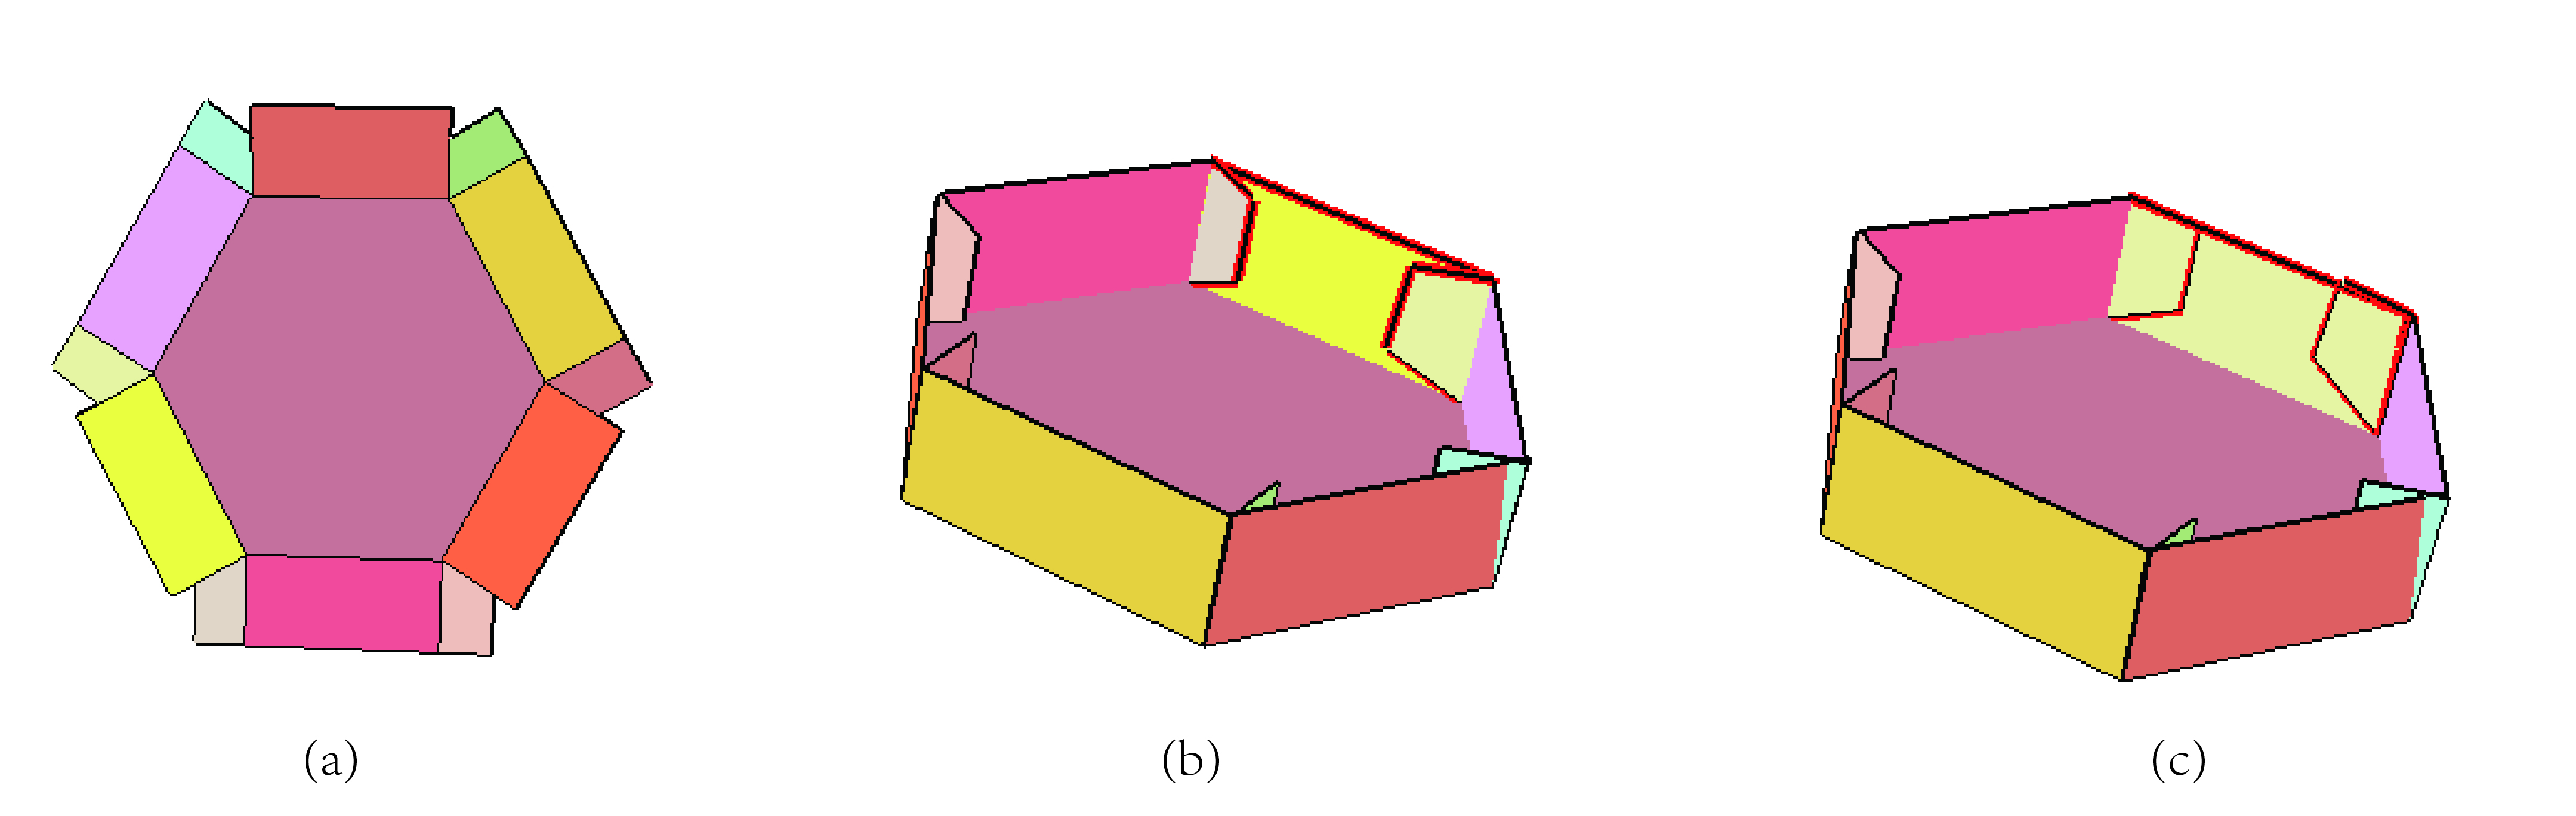
\includegraphics[width=0.9\textwidth]{images/facepaste.jpg}
	\caption{The initialization result (b) of hexagonal box layout (a) can not reach an ideal state by merging vertexes, hence our system allow users to select merging faces which are bounded by red lines (b) and enforce planarity to the model, the result is shown by assigning same color to the coplane faces (c).}
	\label{fig:facepaste}
\end{figure}

\begin{figure}
	\centering
	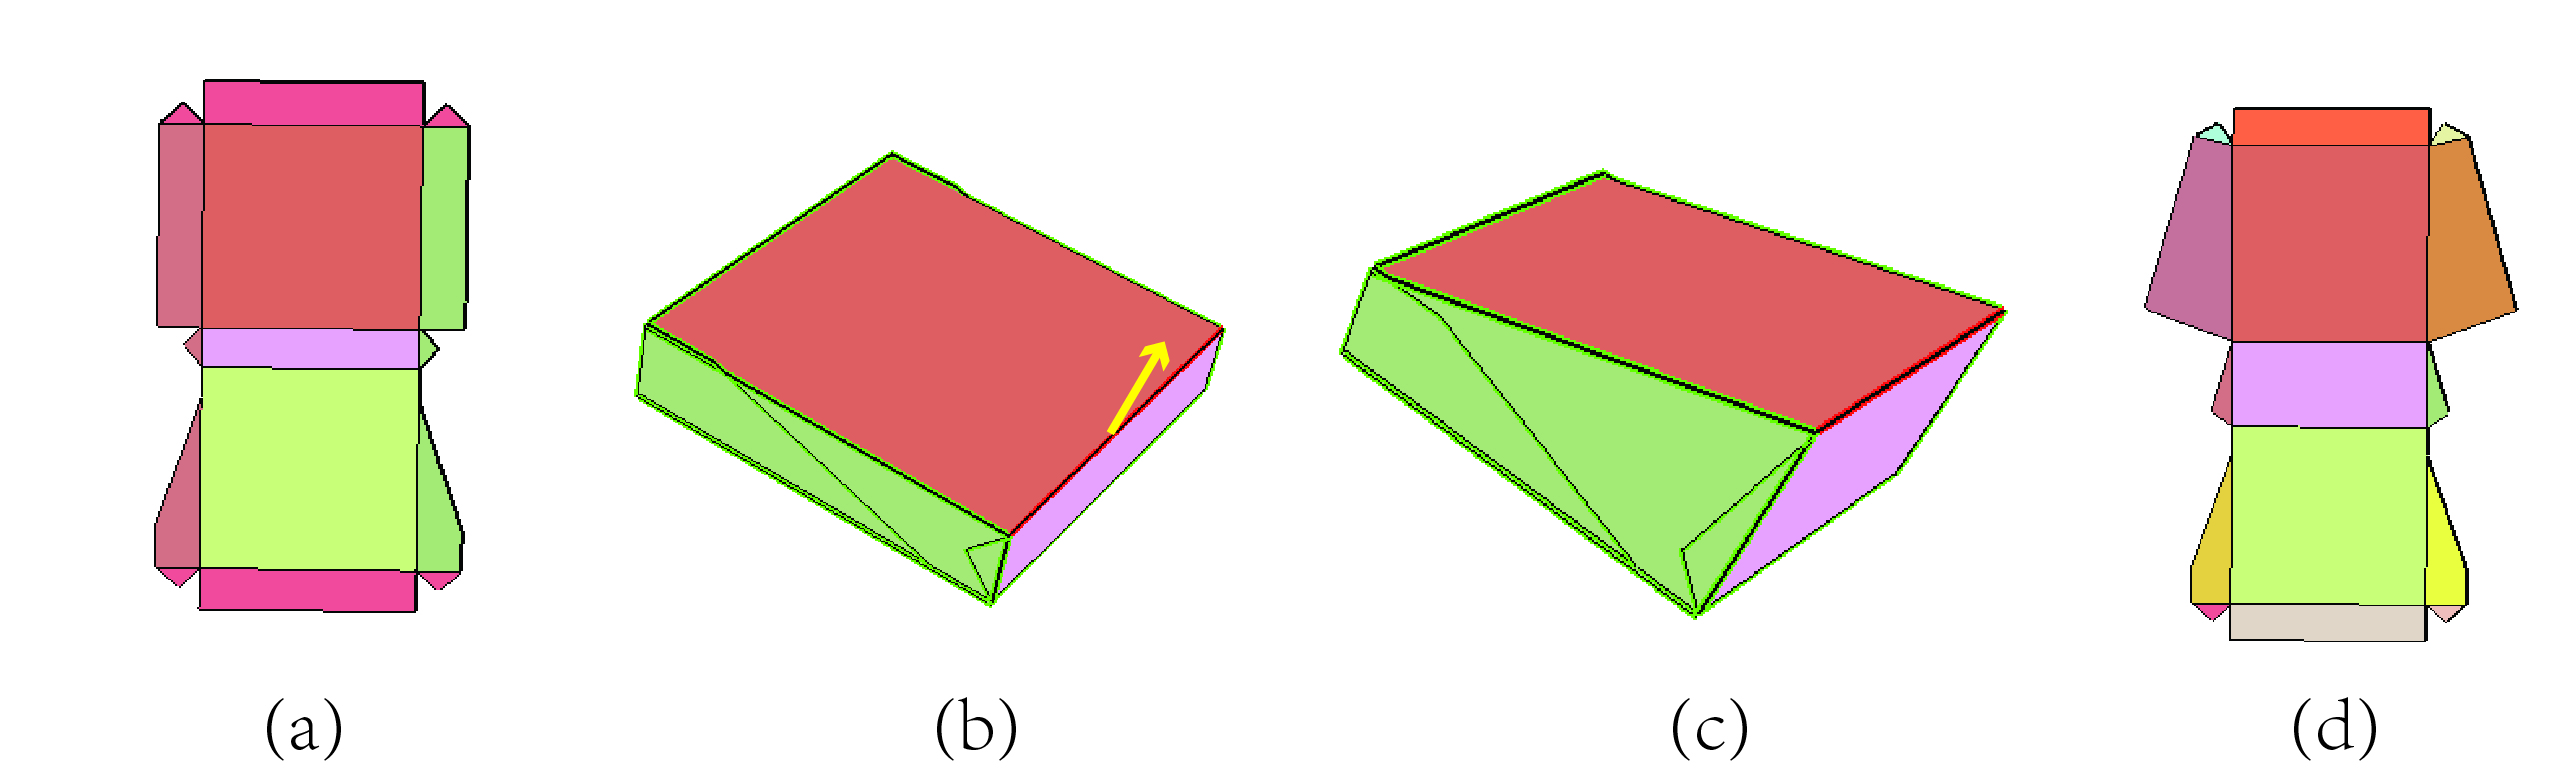
\includegraphics[width=0.9\textwidth]{images/editing.jpg}
	\caption{A standard cuboid carton (b) can be generated by the layout (a). Users are allowed to edit the shape of 3D model by dragging the edges, then the model will be deformed to a novel carton (c), by enforce the constrains to layout, our system can generate a deformable layout automatically as (d) shows.}

\end{figure}
}


\subsection{2D Layout Refinement from 3D Editing}

While it is significantly efficient to generate a 3D carton using our approach from an existing layout, our system allows users to creatively edit the current 3D carton model by moving an edge and simultaneously refine the 2D layout automatically according to the 3D editing.

When the 3D mesh changes, the new shape constraints are transferred to the 2D layouts by keeping face rigidity (Eq.~\ref{equ:plane}).
Since the layout remains in a 2D plane, the coplanarity is enforced for all the vertexes in the layout. 
%
% 
The irrelevant vertexes that do not lie on the moving edge have to stay at their original locations, as described in Eq.~\ref{equ:irrelevant}.
Figure~\ref{fig:editing} shows two examples of automatic layout refinement from 3D editing.                                                                     

\begin{figure}
	\centering
	\subfigure[]{
		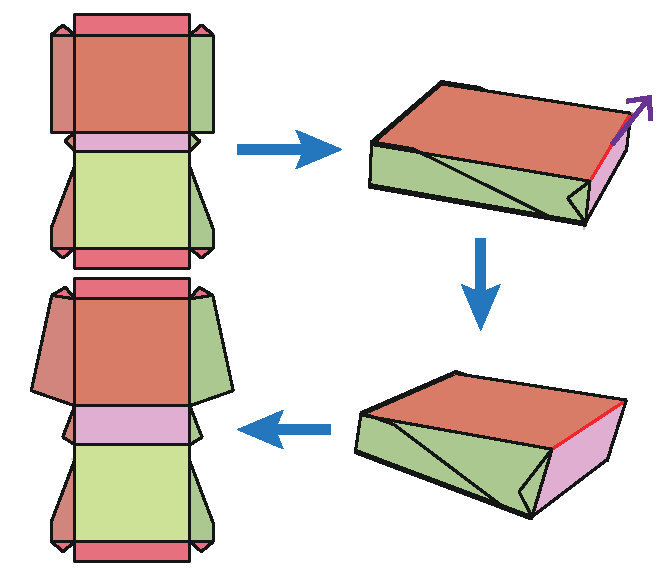
\includegraphics[width=0.45\textwidth]{images/editing1}
		\label{fig:editing1}
	}
	\hfill
	\subfigure[]{
		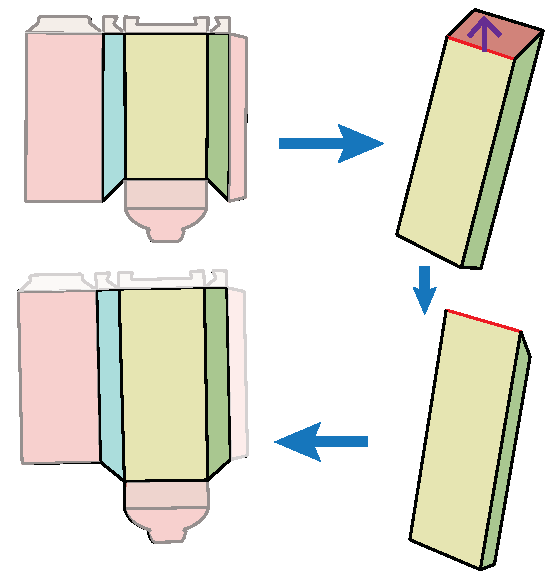
\includegraphics[width=0.45\textwidth]{images/editing2}
		\label{fig:editing2}
	}
	\caption{Two examples of layout modification from 3D model editing. For each example, a box-like carton can be generated from the given 2D layout. Users can edit the shape of the 3D carton by dragging edges in our system. By enforce the shape rigidity constrains, our system automatically updates the 2D layout.}
	\label{fig:editing}
\end{figure}



\section{Results and Discussion}\label{sec:result}
{\color{red}{SS: Any need to list the number of steps we take to generate final model?}}

The step of shape optimization in our paper can be best demonstrated on the model Figure~\ref{fig:result}, through initialization, we can have a rough concept of the final model, and by user interaction including selecting vertexes merged and faces in the same plane, we can finally generate a pleasing model from a given structural layout.

\begin{figure}
	\centering
	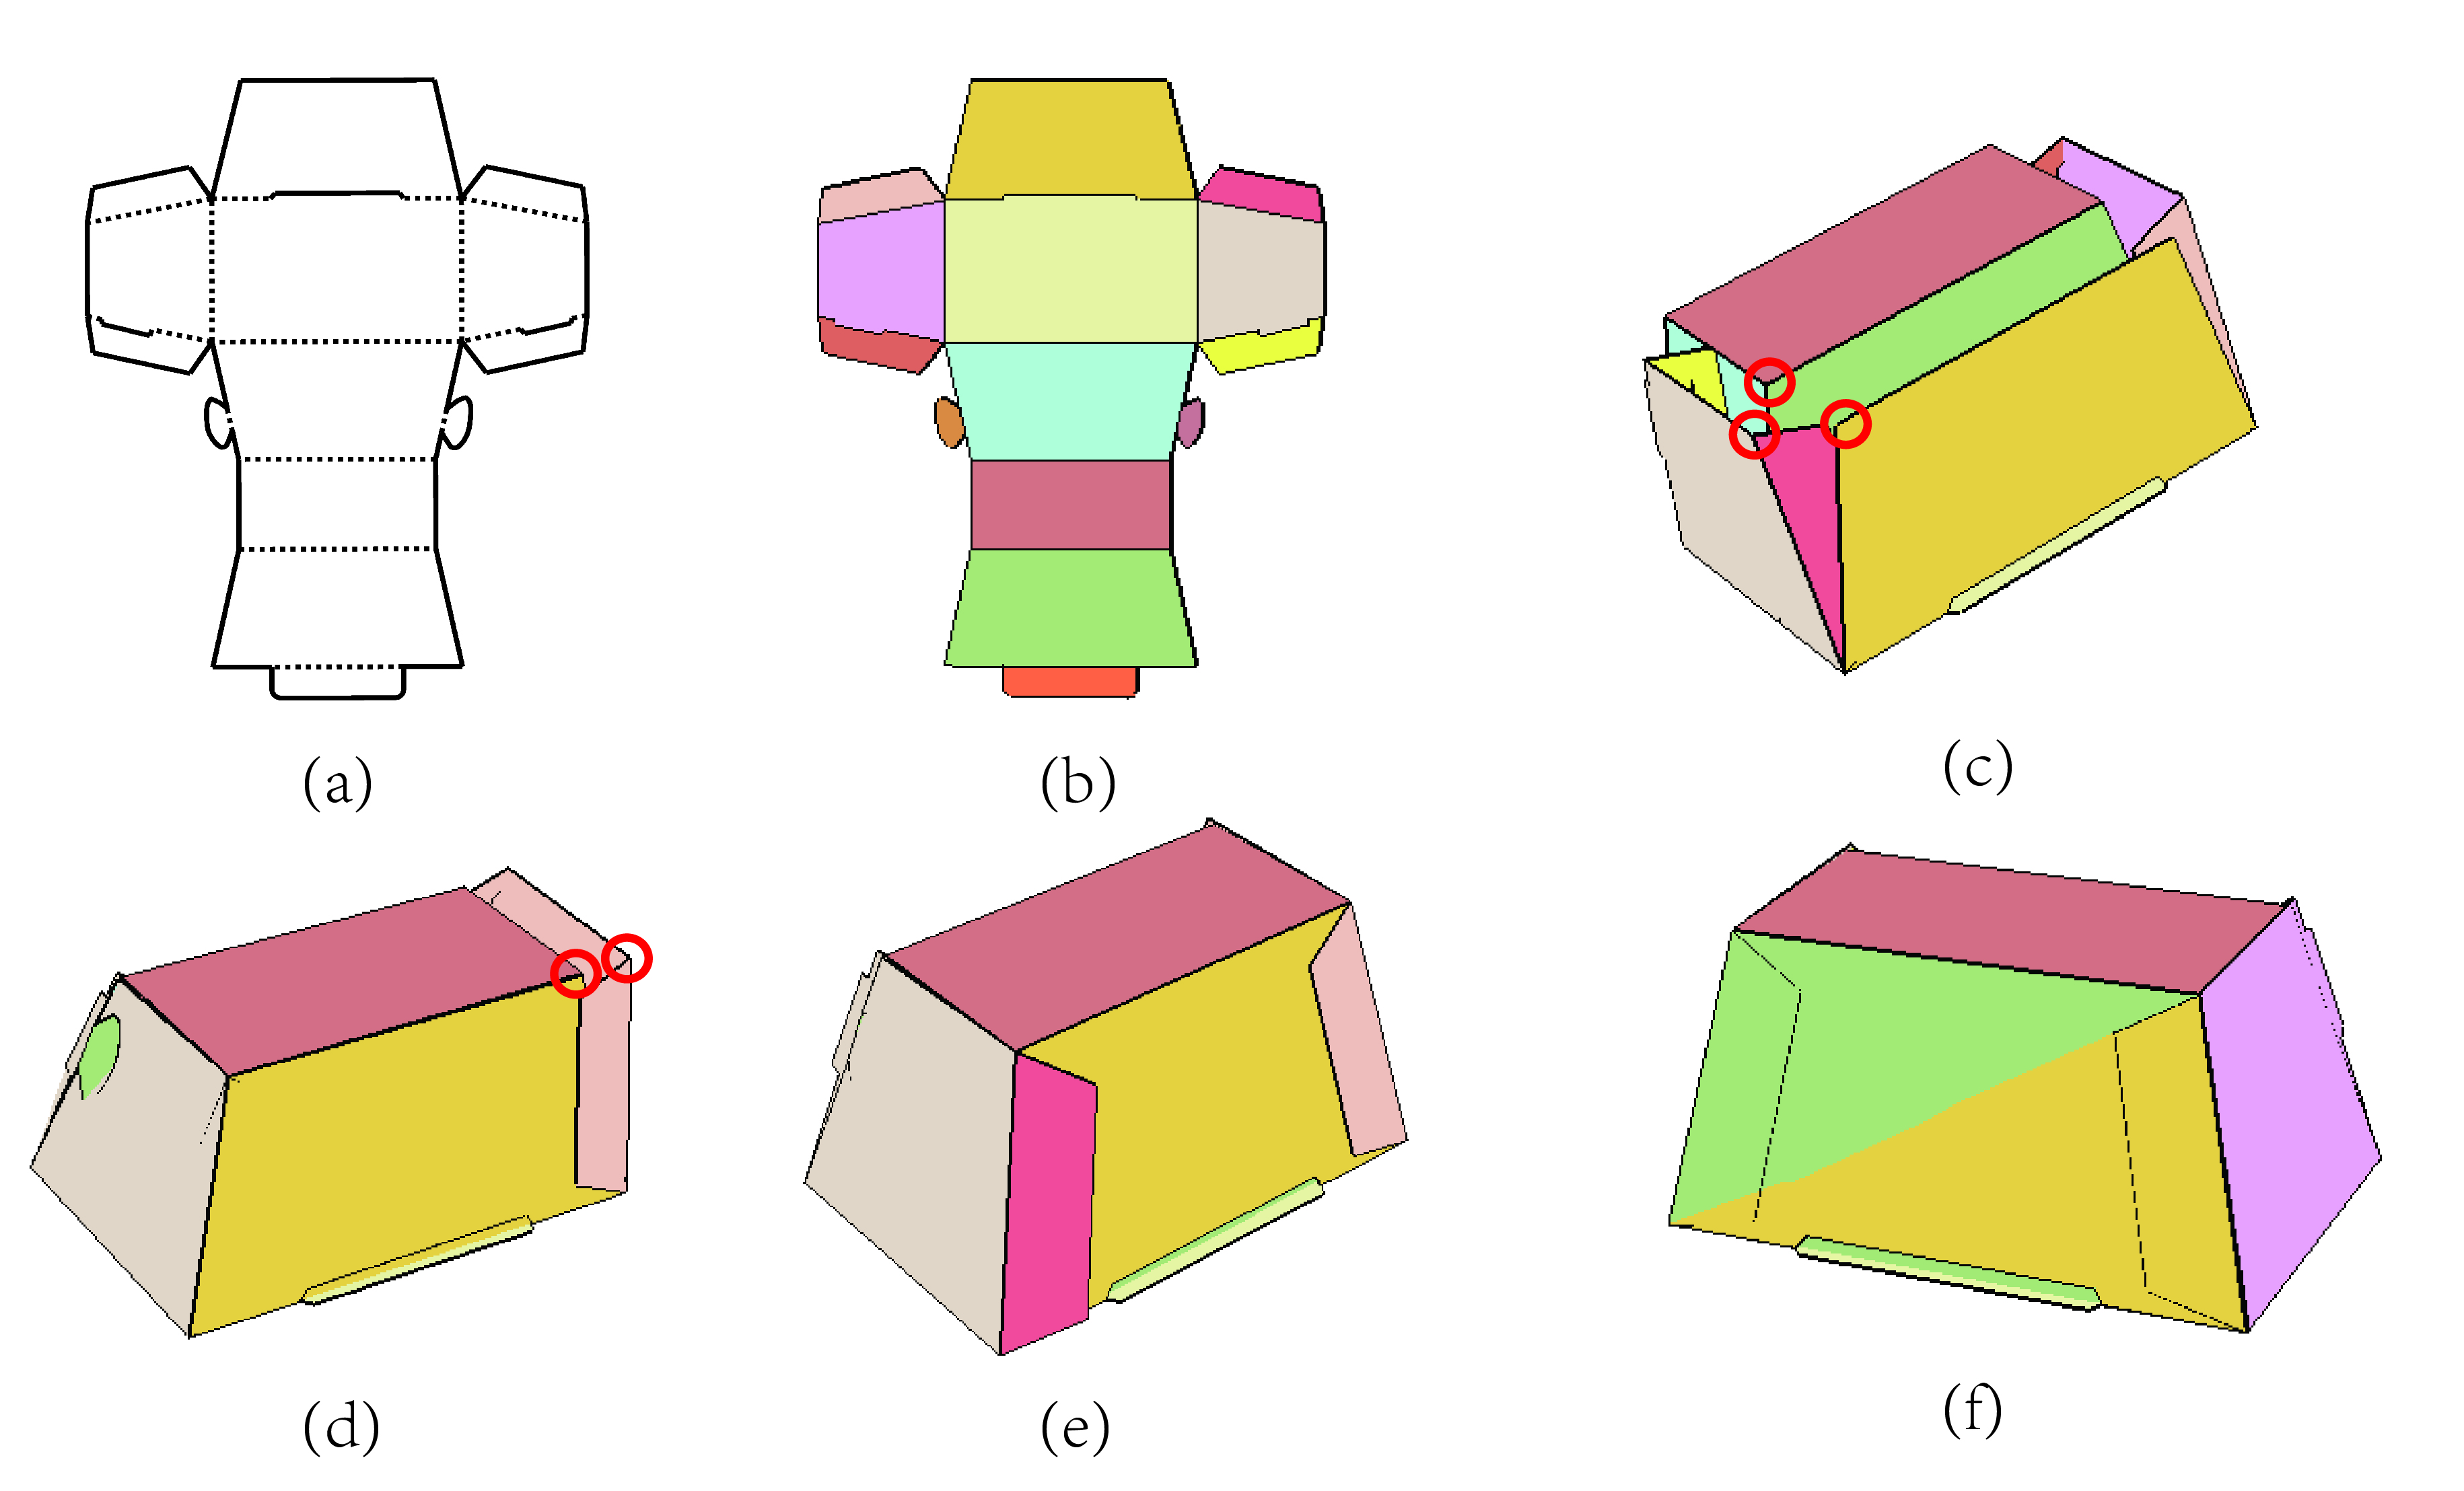
\includegraphics[width=0.9\textwidth]{images/result.jpg}
	\caption{Structural layout (a) is used to generate flat polymesh (b), and then initialize to a rough model (c), after merge the three vertexes in red circles (c) and the two vertexes circled red (d), the model is almost closed with two paste faces in red and pink outside the carton (e), finally through selecting these faces are in the same plane of the yellow face as surface, we can have the final model (f).}
	\label{fig:result}
\end{figure}

We show a number of 3D models generated by our system Figure~\ref{fig:more}, and most of the cases can have an ideal result after initialization because of the cuboid shape as Figure~\ref{fig:more} (a). Through interaction, users can folding more complicated cartons to ideal shapes as Figure~\ref{fig:more} (b).

{\color{blue}{Add table for number of operation steps}}

However, the initialization will not generate a pleasing result on some complicated cases, and leads to the difficult interaction to get the final model. As for Figure~\ref{fig:limitation}, to have a better corresponding model, users need to take at least ten steps to get to Figure~\ref{fig:limitation}(c). 

\begin{figure}
	\centering
	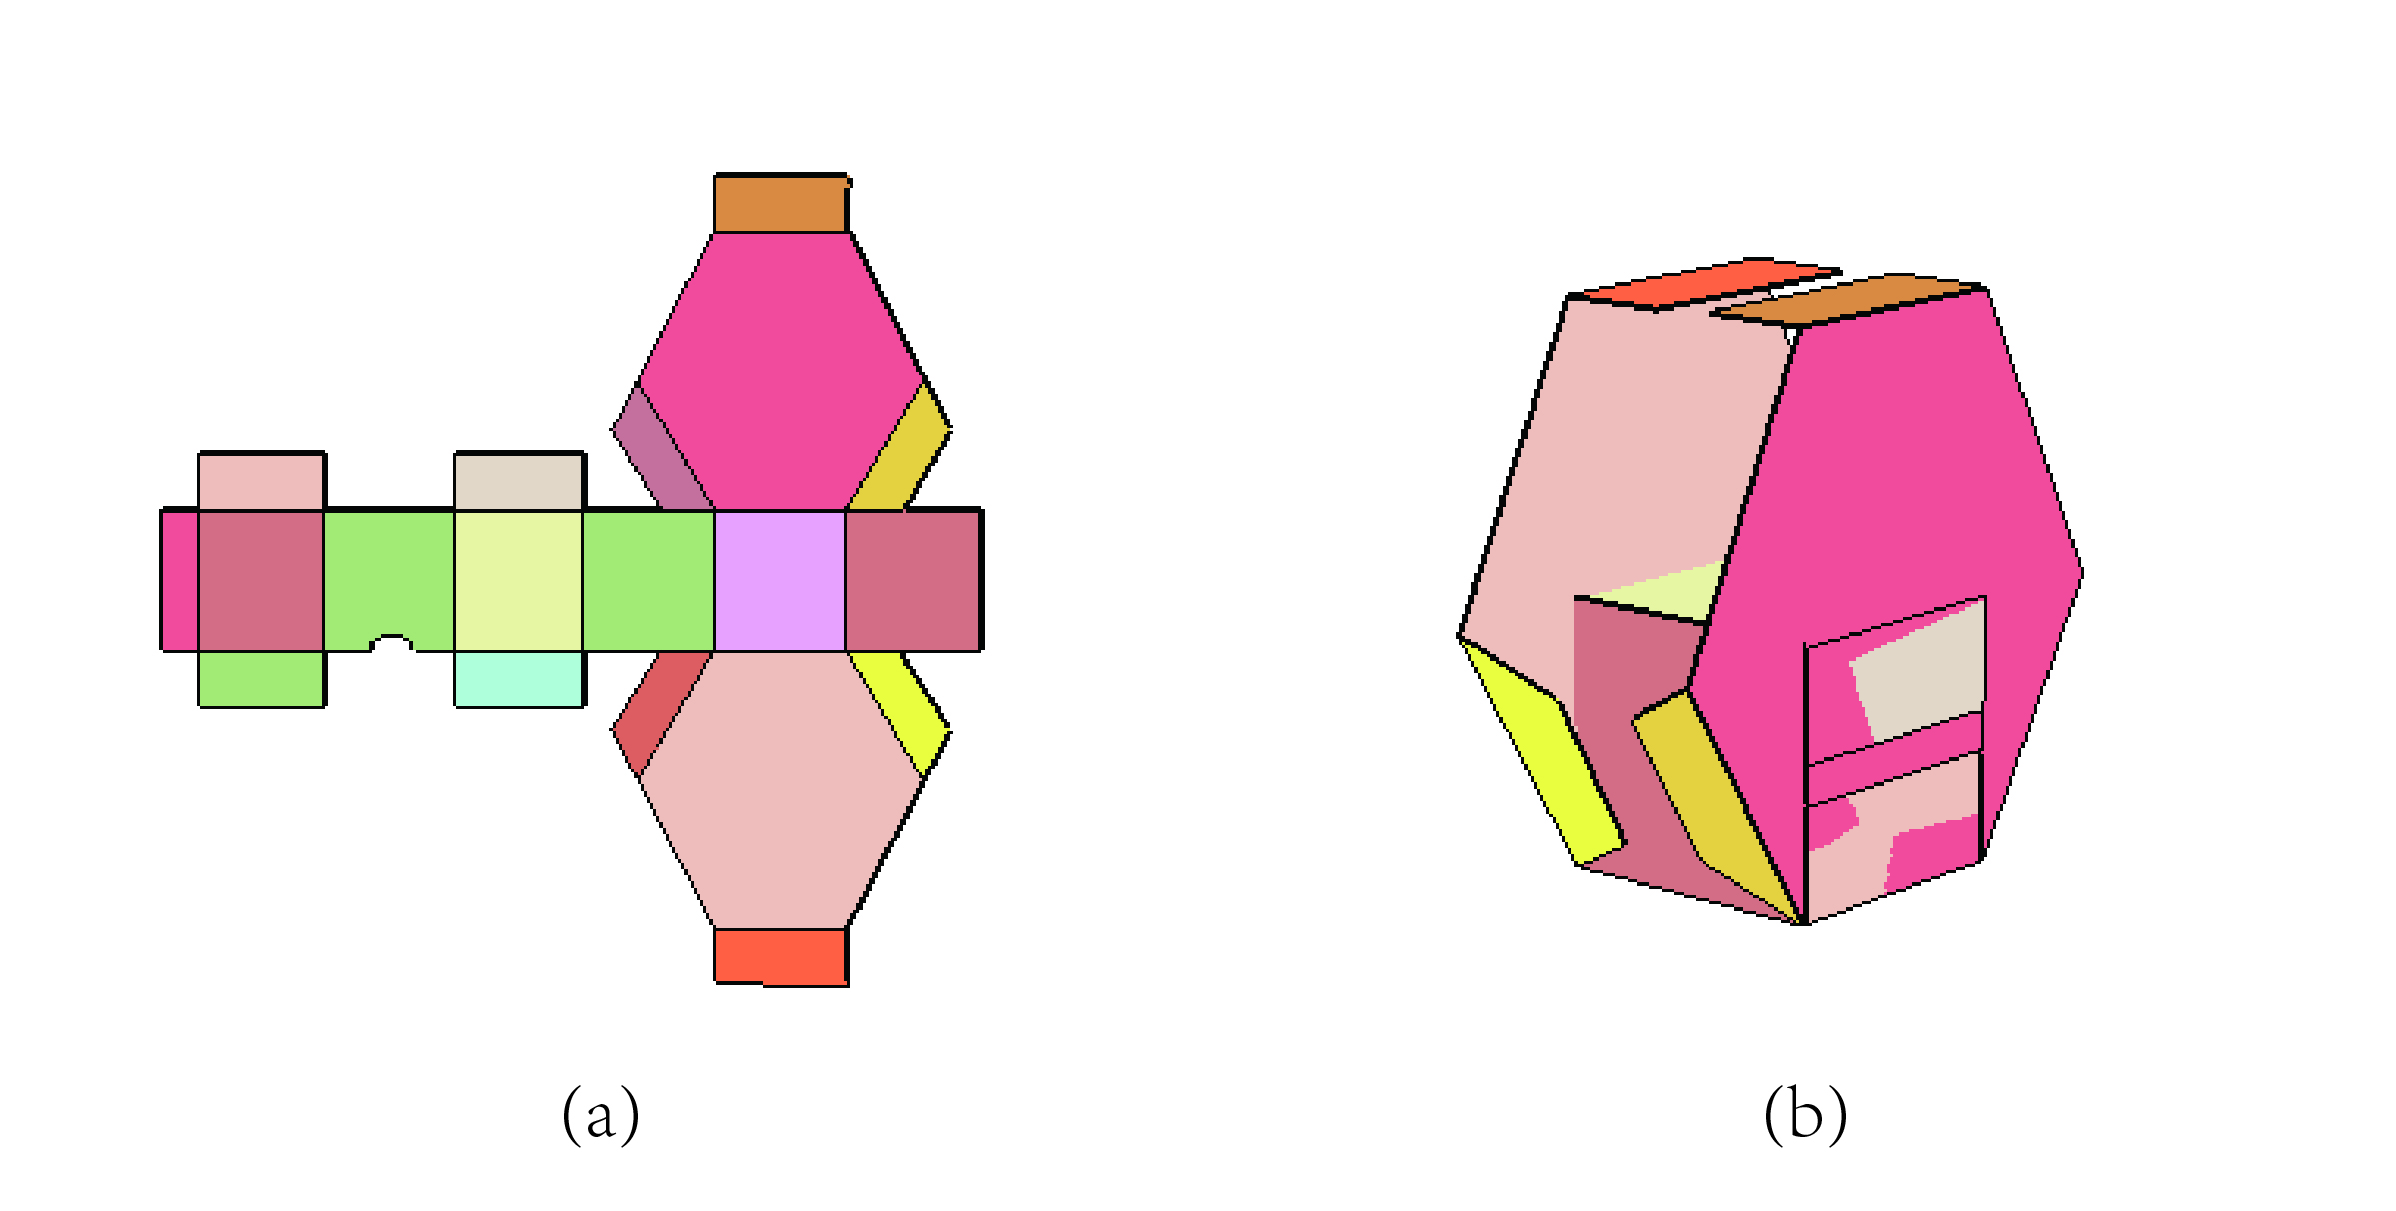
\includegraphics[width=0.9\textwidth]{images/limitation.jpg}
	\caption{Given a layout as (a), our system can generate an initialized result as (b), and through at least ten steps including select vertexes need to be the same place and faces need to be coplane , users can get the final model as (c).}
	\label{fig:limitation}
\end{figure}



\begin{figure}
	\centering
	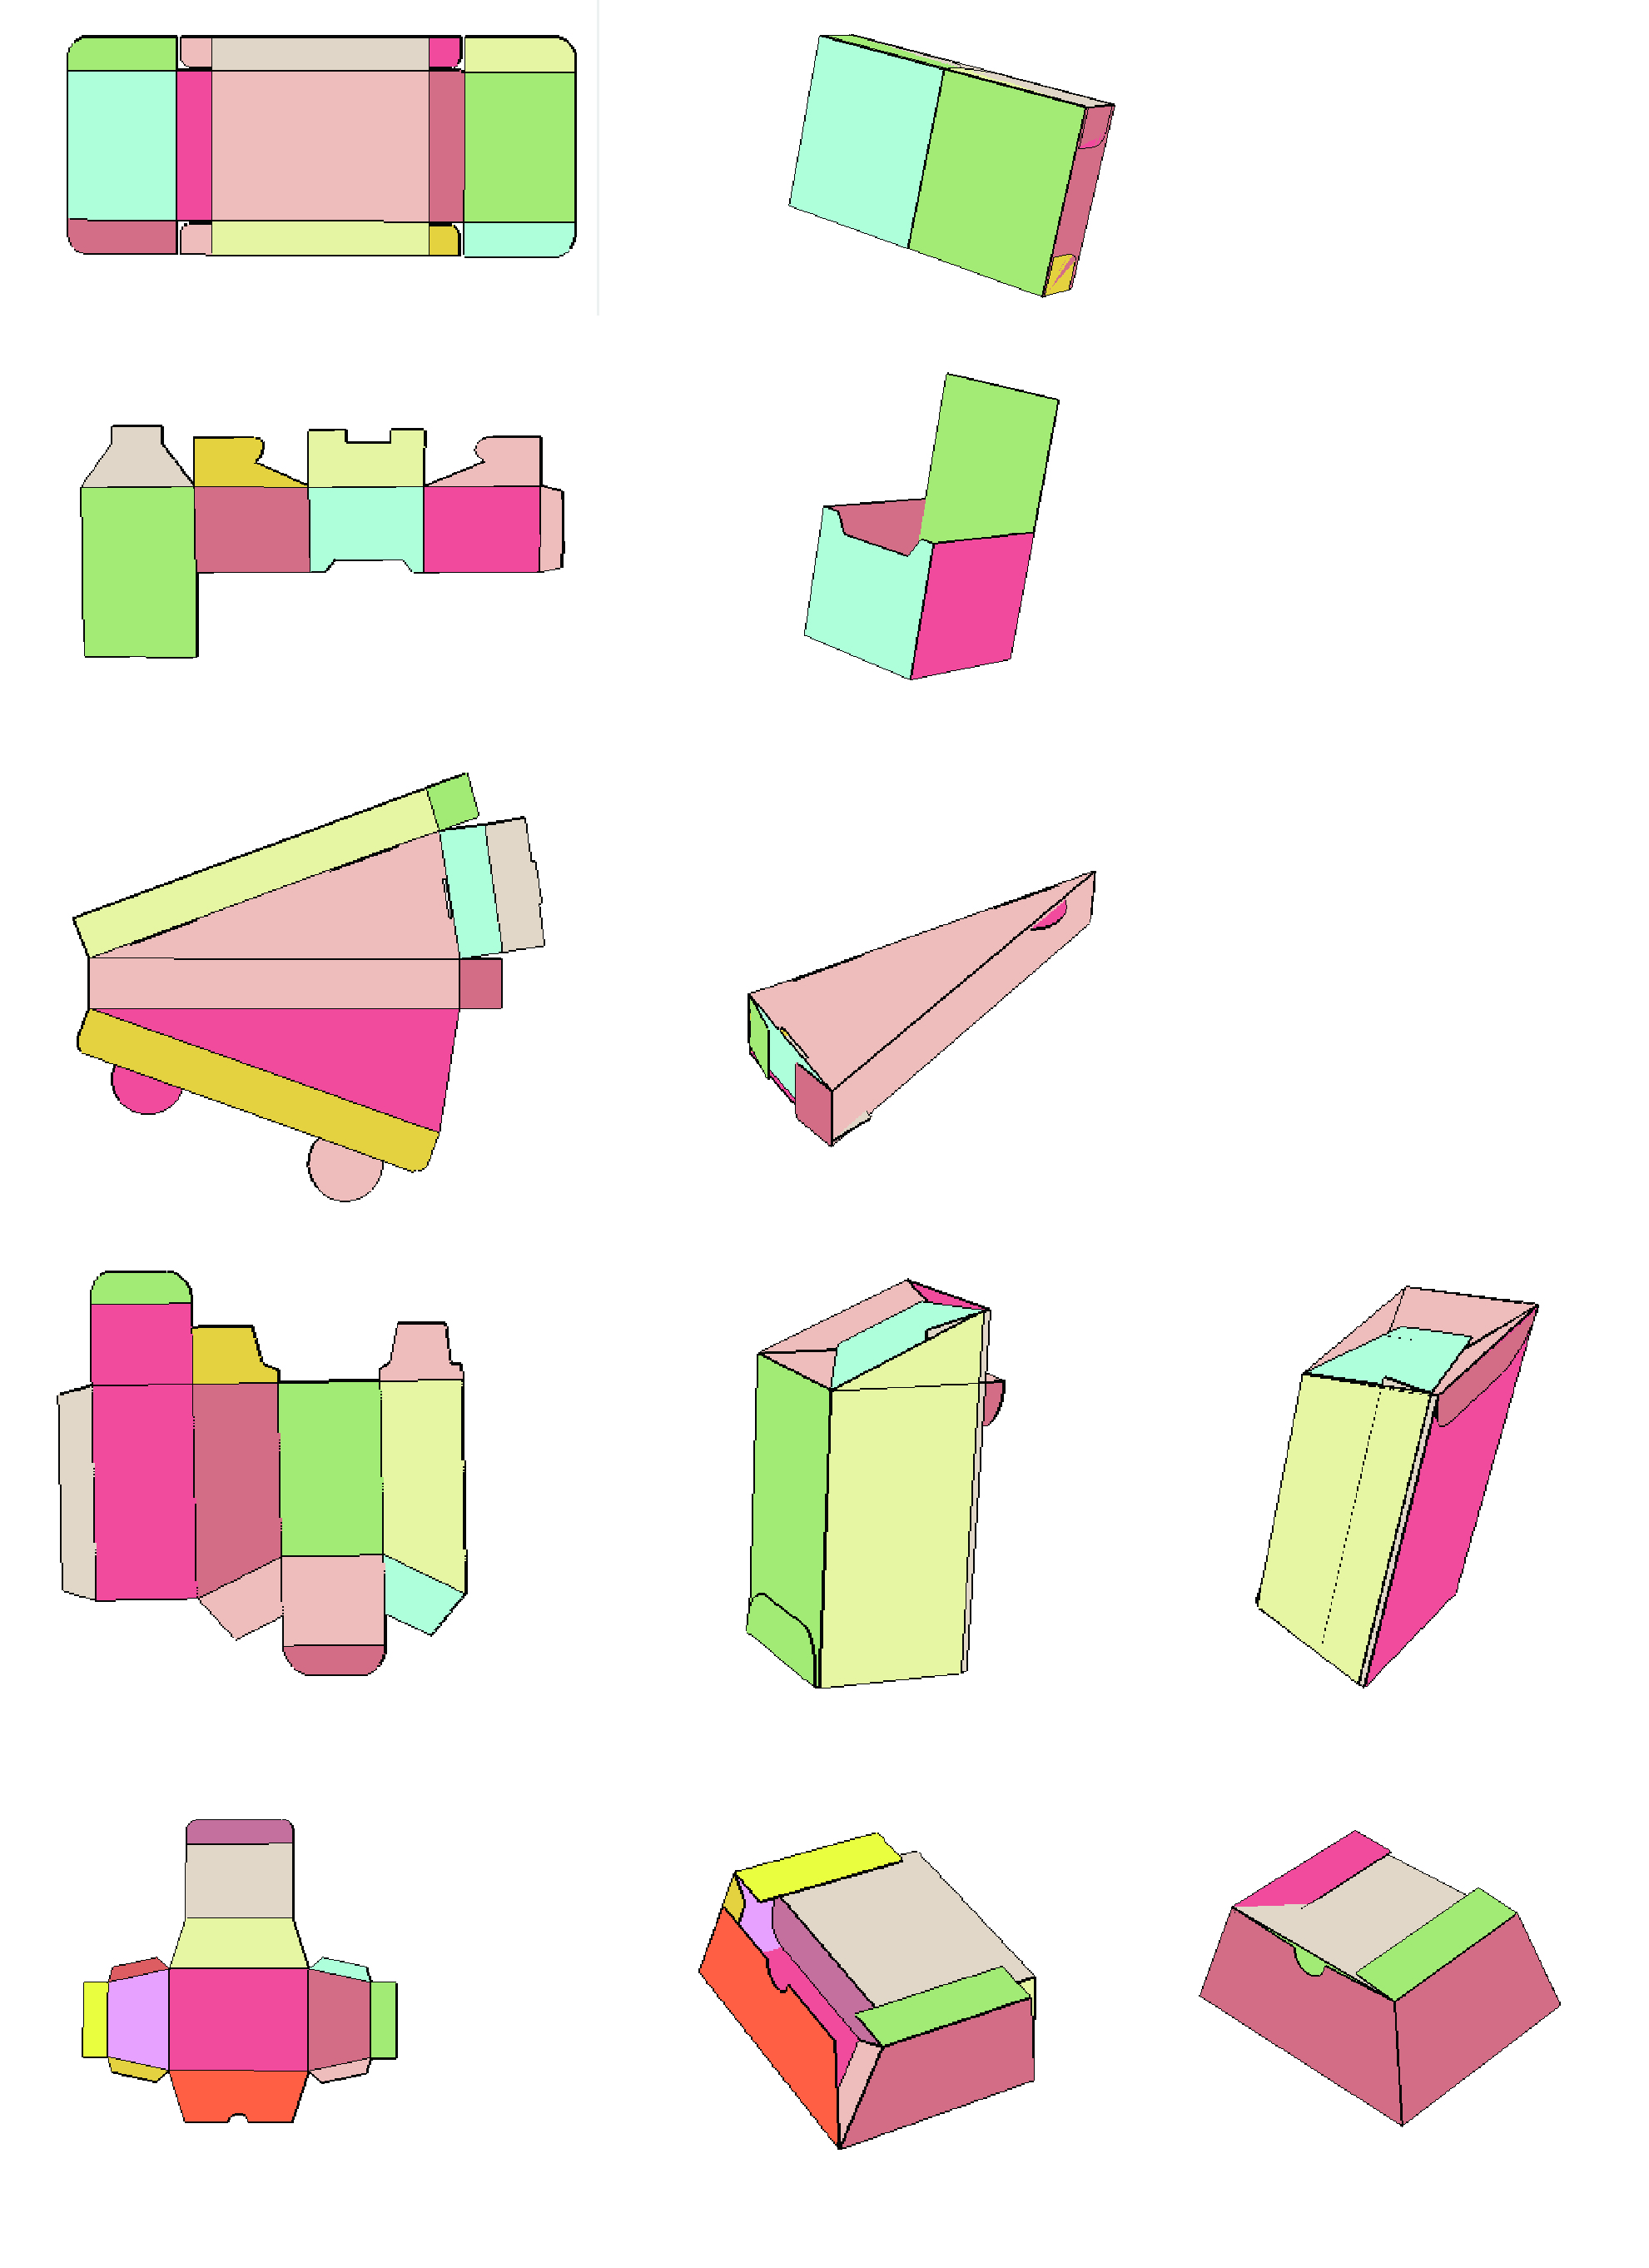
\includegraphics[width=0.9\textwidth]{images/more.jpg}
	\caption{More results, part of cartons can be initialized without refining (a), and with interaction, users can manipulate more complicated cartons (b). The first and second column in (a) and (b) are the flat mesh and initialization result of cartons, and the last column in (b) shows the model after interaction.}
	\label{fig:more}
\end{figure}

%%%%%%%%%%%%%%%%%%%%%%%%%%%%%%%%%%%%%%%%%%%%%%%%%%%%%%%%%%%%%%%%%%%%%

\section{Conclusion and Future Work}\label{sec:conclusion}
In this paper, we present an interactive modeling system to construct a 3D carton model from a 2D expanded layout. 
Based on the automatically folded rough model, a series of shape refinement suggestions are provided for smartly optimizing and editing the carton model, which assists users on producing the desired model efficiently and productively. 
%
Our current system could be further improved in many directions. 
More intelligent editing tools can be implemented. For example, when the user moves a vertex, the vertex translation can be propagated to other symmetric vertexes.
We also would like to improve our automatic folding part with a more comprehensive optimization formulation considering both shape closure and stability. 
%
Moreover, it is desired by designers to support appearance editing in our system.
%

%%%%%%%%%%%%%%%%%%%%%%%%%%%%%%%%%%%%%%%%%%%%%%%%%%%%%%%%%%%%%%%%%%%%

\bibliographystyle{abbrv}
\bibliography{ref}

\end{document}
